%====================================================================
\frame{ \frametitle{Posterior distribution}

  \paragraph{Aim:} Evaluate
  $$
  E[f(\thetabf) | \Ybf]
  $$
  \begin{itemize}
   \item Posterior mean: $f(\thetabf) = \theta_j$
   \item Credibility interval: $f(\thetabf) = \Ibb\{\theta^\ell_j < \theta_j < \theta^u_j\}$
   \item Posterior variance: $f(\thetabf) = \theta_j^2$ \qquad (+ posterior mean)
   \item Posterior covariance: $f(\thetabf) = \theta_j \theta_k$ \qquad (+ posterior means)
  \end{itemize}

  \bigskip \bigskip \pause
  \paragraph{Main problem:} evaluate
  $$
  p(\thetabf \gv \Ybf) = \frac{\pi(\thetabf) \bf \ell(\Ybf \gv \thetabf)}{p(\Ybf)}
  $$
  which requires to evaluate
  $$
  p(\Ybf) = \int \underset{prior}{\underbrace{\pi(\thetabf)}} \; \underset{likelihood}{\underbrace{\ell(\Ybf \gv \thetabf)}} \d \thetabf
  $$
}

%====================================================================
\subsection{Conjugate priors}
\frame{\frametitle{Outline} \tableofcontents[currentsubsection]}
%====================================================================
\frame{ \frametitle{Nice case: Conjugate priors}

  \paragraph{Example: Bernoulli}\footnote{\#\ref{slide:prior}: from top to bottom, $(a, b) = (1, 10), (5, 5), (1, 1)$}
  \begin{description}
   \item[Prior:] $\theta =$ probability to carry a disease. 
   $$
   \theta \sim \Beta(a, b), 
   \qquad 
   \pi(\theta) \propto \theta^{a-1} (1-\theta)^{b-1}
   $$ \pause
   \item[Likelihood:] $Y_i = 1$ if disease, $0$ otherwise. $S =$ number of carriers
   $$
   Y_i \gv \theta \sim \Bcal(\theta), 
   \qquad 
   \ell(\Ybf \gv \theta) = \prod_i \theta^{Y_i} (1-\theta)^{1-Y_i} = \theta^{S} (1-\theta)^{n-S}
   $$ \pause
   \item[Posterior:]
   $$
   p(\theta \gv \Ybf) \propto \pi(\theta) \ell(\Ybf \gv \theta) = \theta^{a+S-1} (1-\theta)^{b+n-S-1}
   $$
   which means that
   $$
   \theta \gv \Ybf \sim \Beta(a+S, b+n-S)
   $$
  \end{description}
}

%====================================================================
\frame{ \frametitle{Conjugate priors: Discrete distributions}

  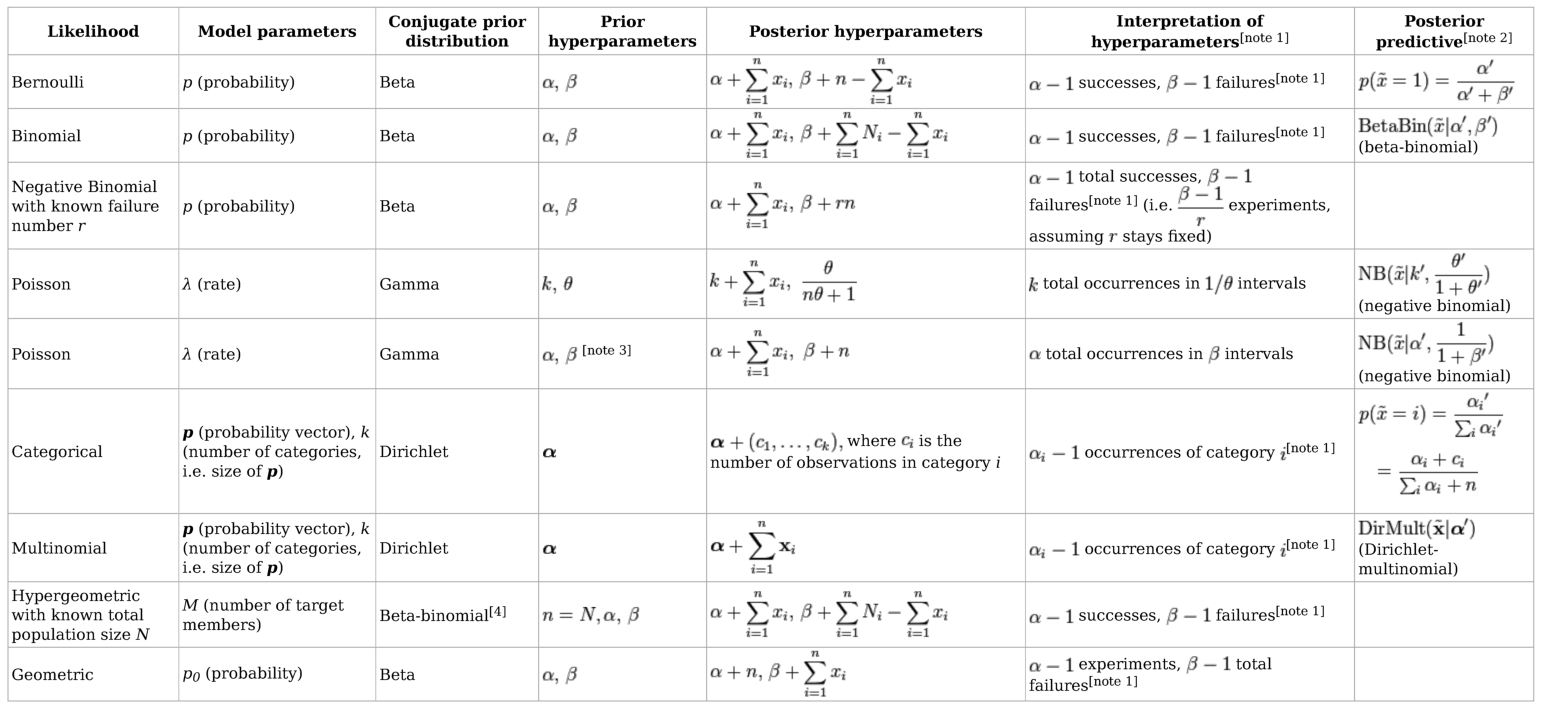
\includegraphics[width=1\textwidth]{../figs/WikipediaConjugatePrior-Discrete}

  \footnotesize{\url{en.wikipedia.org/wiki/Conjugate_prior}}
}

%====================================================================
\frame{ \frametitle{Conjugate priors: Continuous distributions}

  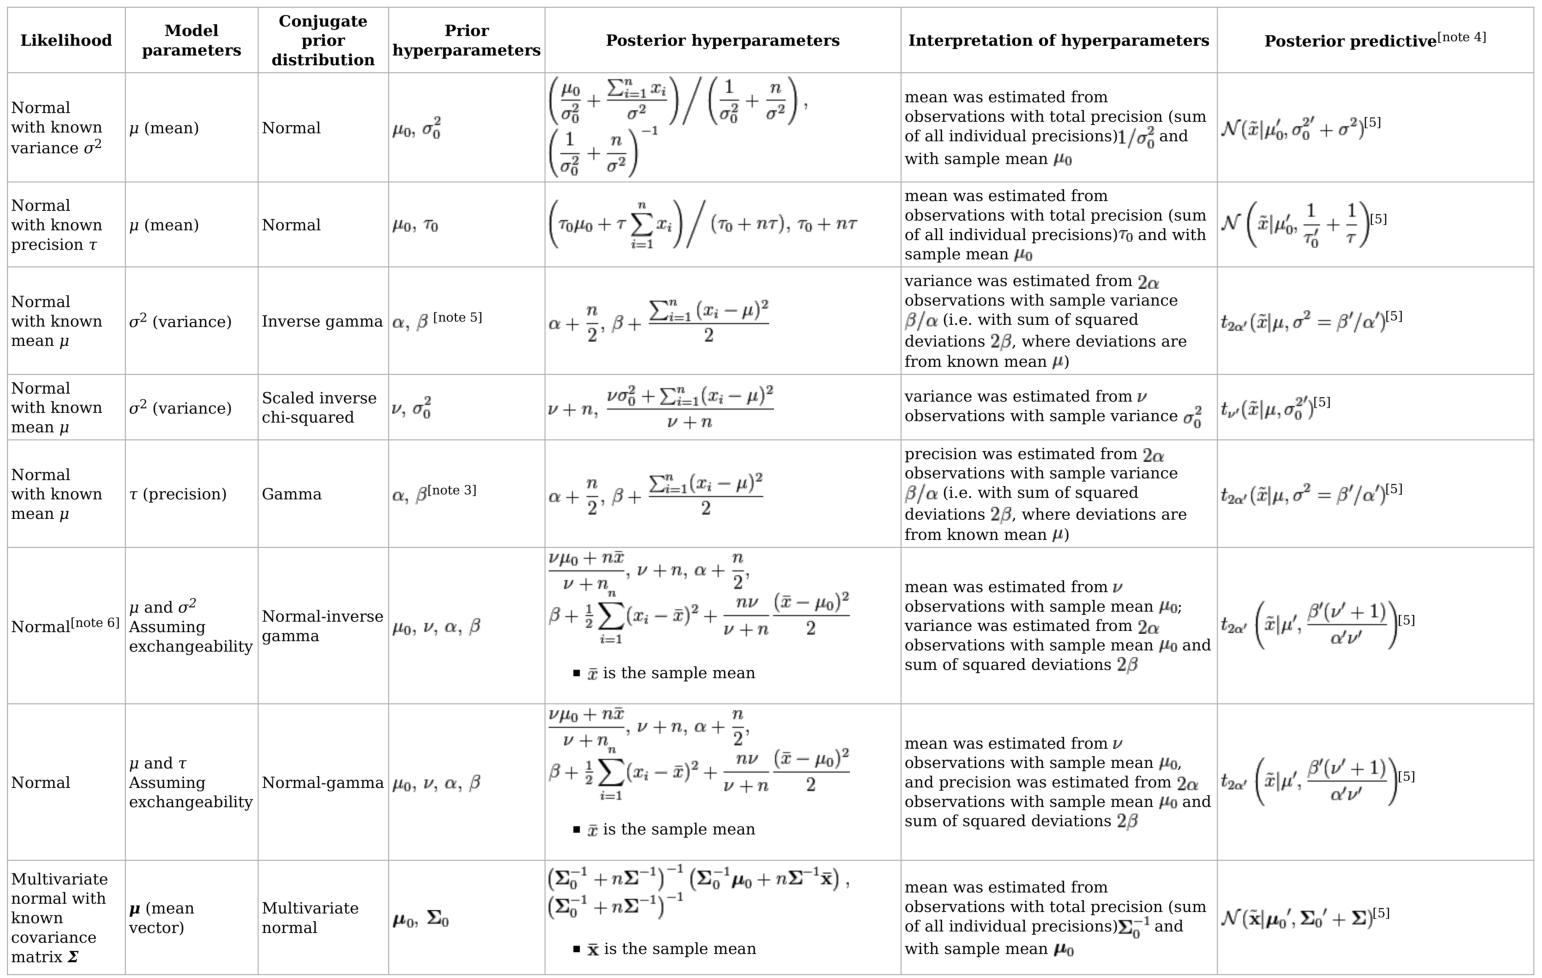
\includegraphics[width=1\textwidth]{../figs/WikipediaConjugatePrior-Continuous}

  \footnotesize{\url{en.wikipedia.org/wiki/Conjugate_prior}}
}

%====================================================================
\subsection{Monte Carlo integration}
\frame{\frametitle{Outline} \tableofcontents[currentsubsection]}
%====================================================================
\frame{ \frametitle{Computing integrals}

  \paragraph{General case:} $p(\thetabf \gv \Ybf)$ has no close form
  
  \bigskip 
  \paragraph{Goal:} compute
  $$
  \Esp(f(\thetabf) \gv \Ybf) 
  = \int f(\thetabf) p(\thetabf \gv \Ybf) \d \thetabf
  = \left. \int f(\thetabf) \pi(\thetabf) \; \ell(\Ybf \gv \thetabf) \d \thetabf \right/ p(\Ybf) 
  $$
  where
  $$
  p(\Ybf) = \int \pi(\thetabf) \; \ell(\Ybf \gv \thetabf) \d \thetabf 
  $$
  
  \bigskip \bigskip \pause
  We need to evaluate integrals of the form
  $$
  \int [\cdots] \; \emphase{\pi(\thetabf) \; \ell(\Ybf \gv \thetabf)} \d \thetabf 
  $$
}

%====================================================================
\frame{ \frametitle{Monte Carlo}

  \paragraph{Principle.} To evaluate
  $$
  \Esp_q[f(\thetabf)] = \int f(\thetabf) \emphase{q(\thetabf)} \d \thetabf
  $$
  \begin{enumerate}
   \item \pause sample 
   $$
   (\thetabf^1, \dots, \thetabf^B) \text{ iid } \sim q
   $$
   \item \pause compute
   $$
   \widehat{\Esp}_q[f(\thetabf)] = \frac1B \sum_b f(\thetabf^b)
   $$
  \end{enumerate}
  \pause \ra unbiased estimate of $\Esp_q[f(\thetabf)]$ with variance $\propto 1/ B$. \appref{app:MCillustration} \label{back:MCillustration}
  
  \bigskip \bigskip \pause
  \paragraph{In practice:} 
  \begin{itemize}
   \item Works fine to evaluate $\Esp[f(\thetabf)]$, taking $q(\thetabf) = \pi(\thetabf)$
   $$
   \widehat{\Esp}_{\Ncal(0, 10)}\left(e^\theta\right) = \text{\tt mean(exp(rnorm(B, mean=0, sd=sqrt(10))))}
   $$\pause
   \item Useless for $\Esp[f(\thetabf) | \Ybf]$ as we do not know how to sample from $q(\thetabf) = p(\thetabf \gv \Ybf)$
  \end{itemize}
}

%===================================================================
\frame{ \frametitle{Importance Sampling (IS)}

  \paragraph{Main trick = weighting particles.} \pause To evaluate $\Esp[f(\thetabf)]$, write it as
  \begin{align*}
  \Esp_q[f(\thetabf)] 
  = \int f(\thetabf) \emphase{q(\thetabf)} \d \thetabf 
  = \int f(\thetabf) \frac{q(\thetabf)}{q'(\thetabf)} \emphase{q'(\thetabf)} \d \thetabf 
  \end{align*}
  for some \emphase{proposal} $q' \gg q$, from which you {\sl know how to sample}, then
  \begin{enumerate}
   \item \pause sample
   $$
   (\thetabf^1, \dots, \thetabf^B) \text{ iid } \sim \emphase{q'}(\thetabf),
   $$
   \item \pause compute the weights
   $$
   W(\thetabf^b) = q(\thetabf^b) / q'(\thetabf^b), 
   $$
   \item \pause and compute
   $$
   \widehat{\Esp}[f(\thetabf)] = \frac1B \sum_b W(\thetabf^b) f(\thetabf^b)
   $$
  \end{enumerate}
  \pause \ra unbiased estimate of $\Esp[f(\thetabf)]$ with variance $\propto \sum_b W(\theta^b)^2 / B$.

}  

%===================================================================
\frame{ \frametitle{Importance Sampling (a picture)}

  \begin{tabular}{cc}
    \begin{tabular}{p{.3\textwidth}}
	 \onslide+<4>{
	   Efficiency of sampling:
	   $$
	   ESS = \overline{W}^2 / \overline{W^2}
	   $$

	   \bigskip
	   $q' = q$
	   $$
	   \Rightarrow \quad ESS = 1
	   $$
	   }
    \end{tabular}
    & 
%     \hspace{-.\textwidth}
    \begin{tabular}{p{.5\textwidth}}
	 \begin{overprint}
	 \onslide<1>
	 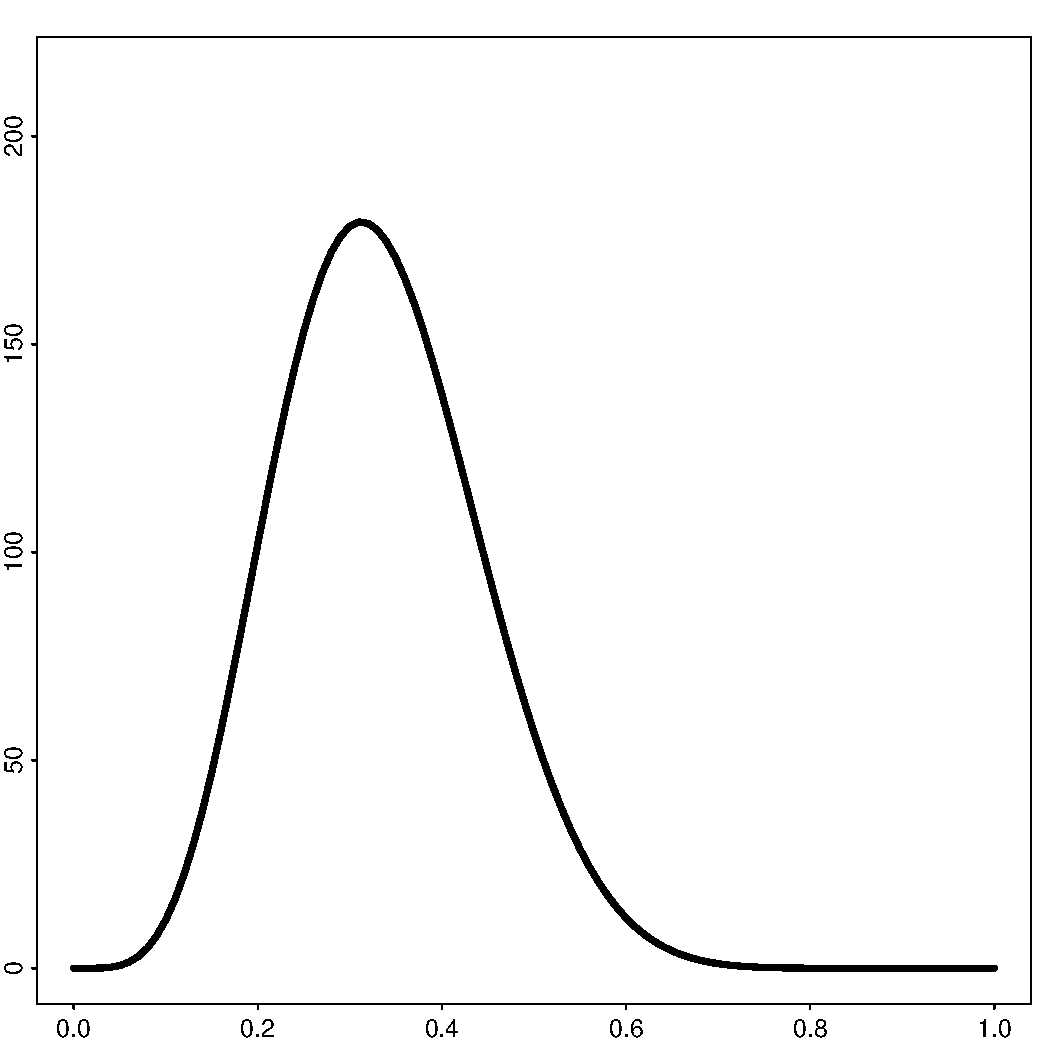
\includegraphics[height=.7\textheight]{../figs/ImportanceSampling-1}
	 \onslide<2>
	 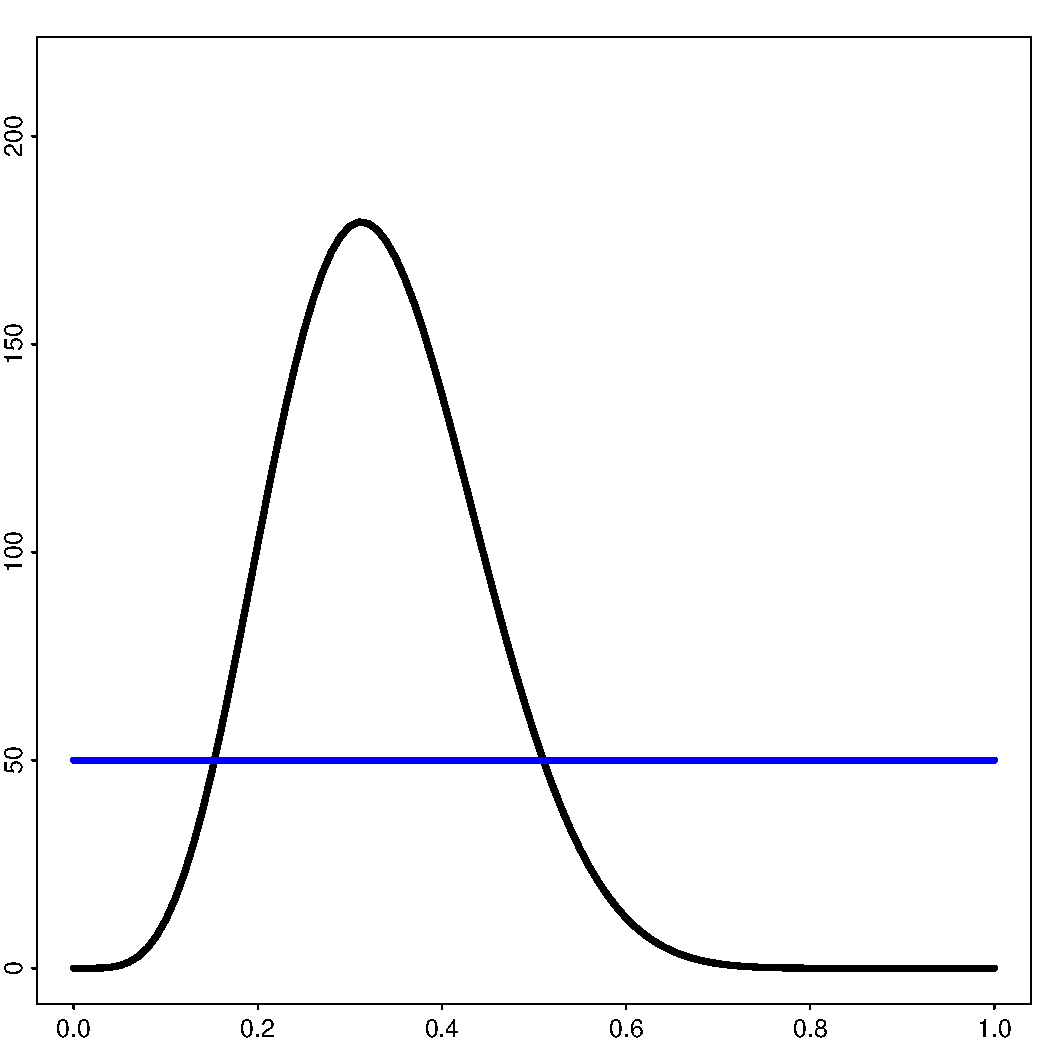
\includegraphics[height=.7\textheight]{../figs/ImportanceSampling-2}
	 \onslide<3>
	 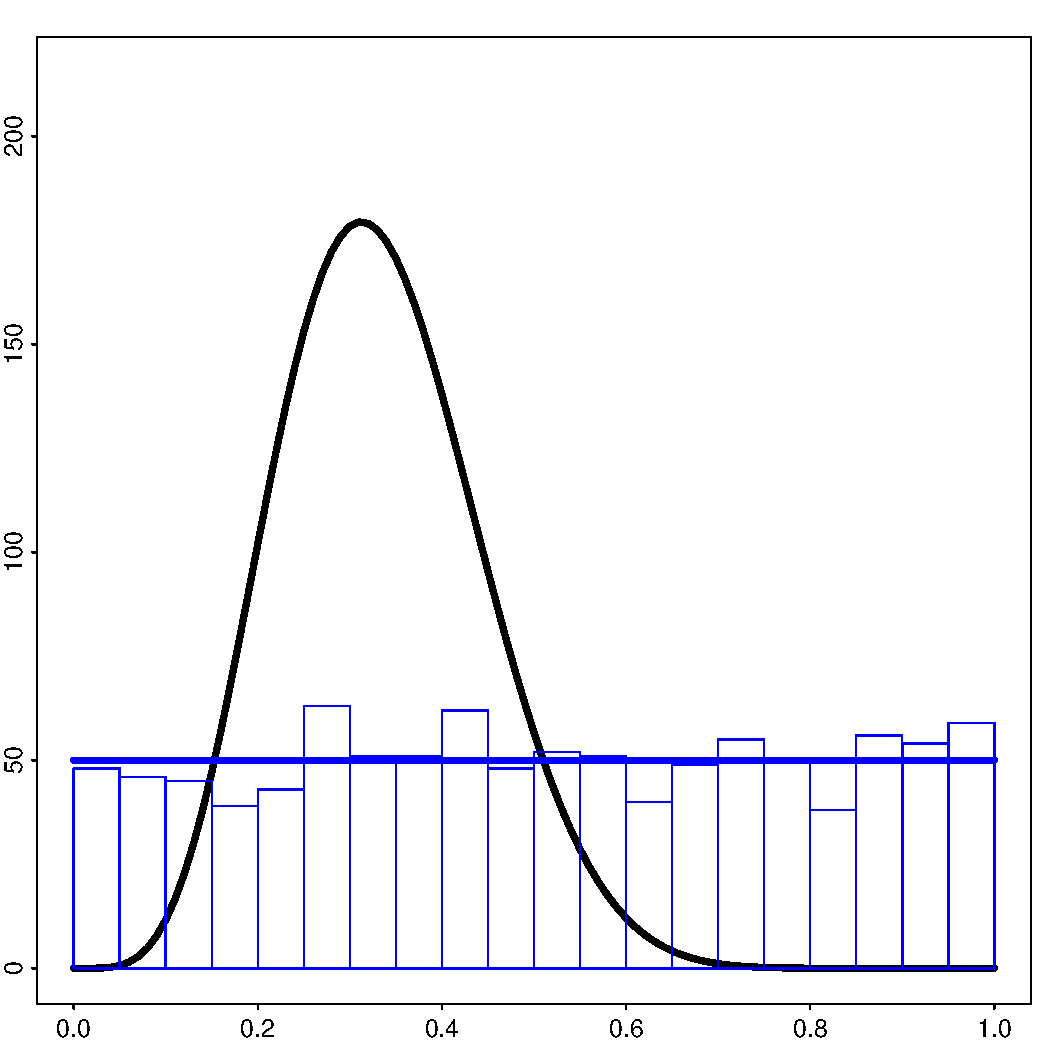
\includegraphics[height=.7\textheight]{../figs/ImportanceSampling-3}
	 \onslide<4>
	 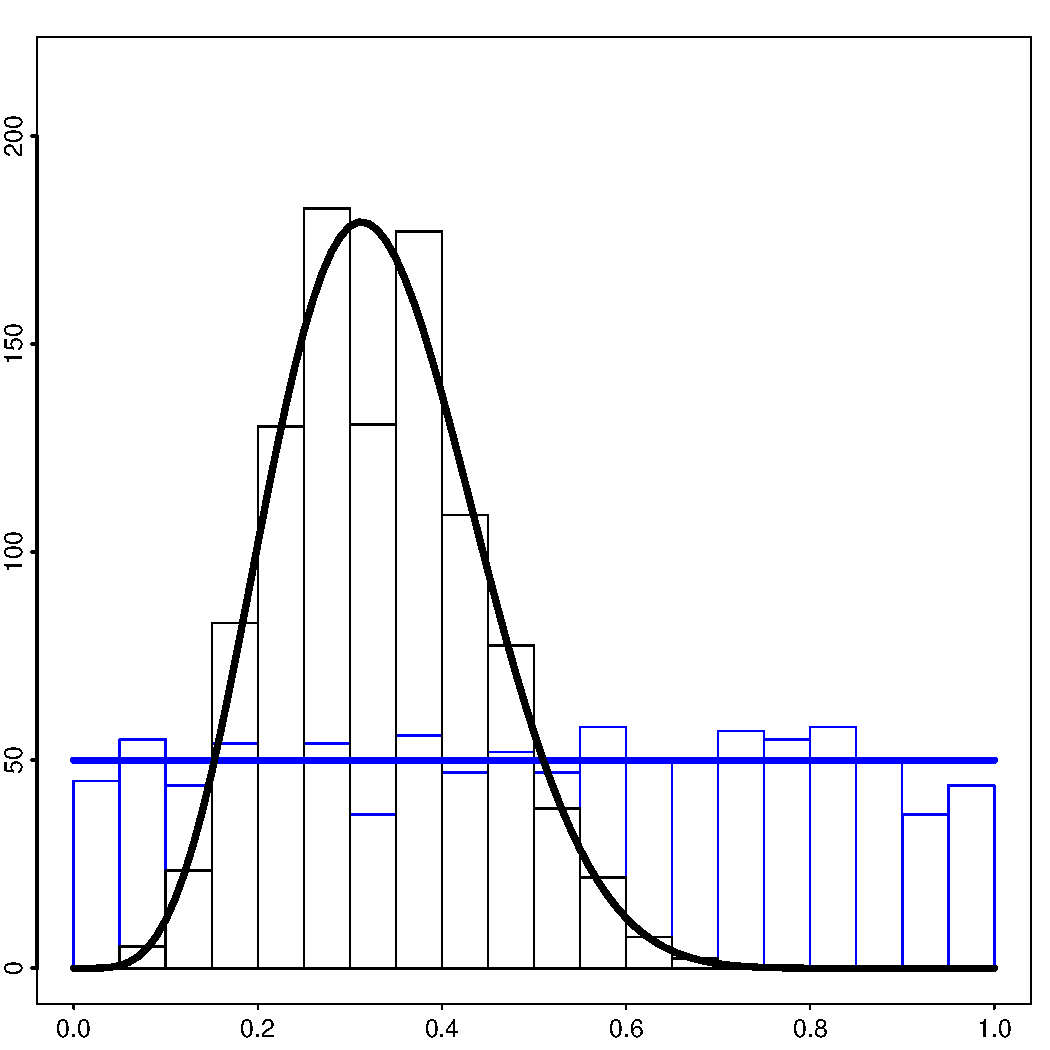
\includegraphics[height=.7\textheight]{../figs/ImportanceSampling-4}
	 \end{overprint}
    \end{tabular}
  \end{tabular}

}  


%===================================================================
\frame{ \frametitle{Importance Sampling: Importance of the proposal}

%   \begin{center}
%   \begin{tabular}{cc}
%     \begin{tabular}{c}
%     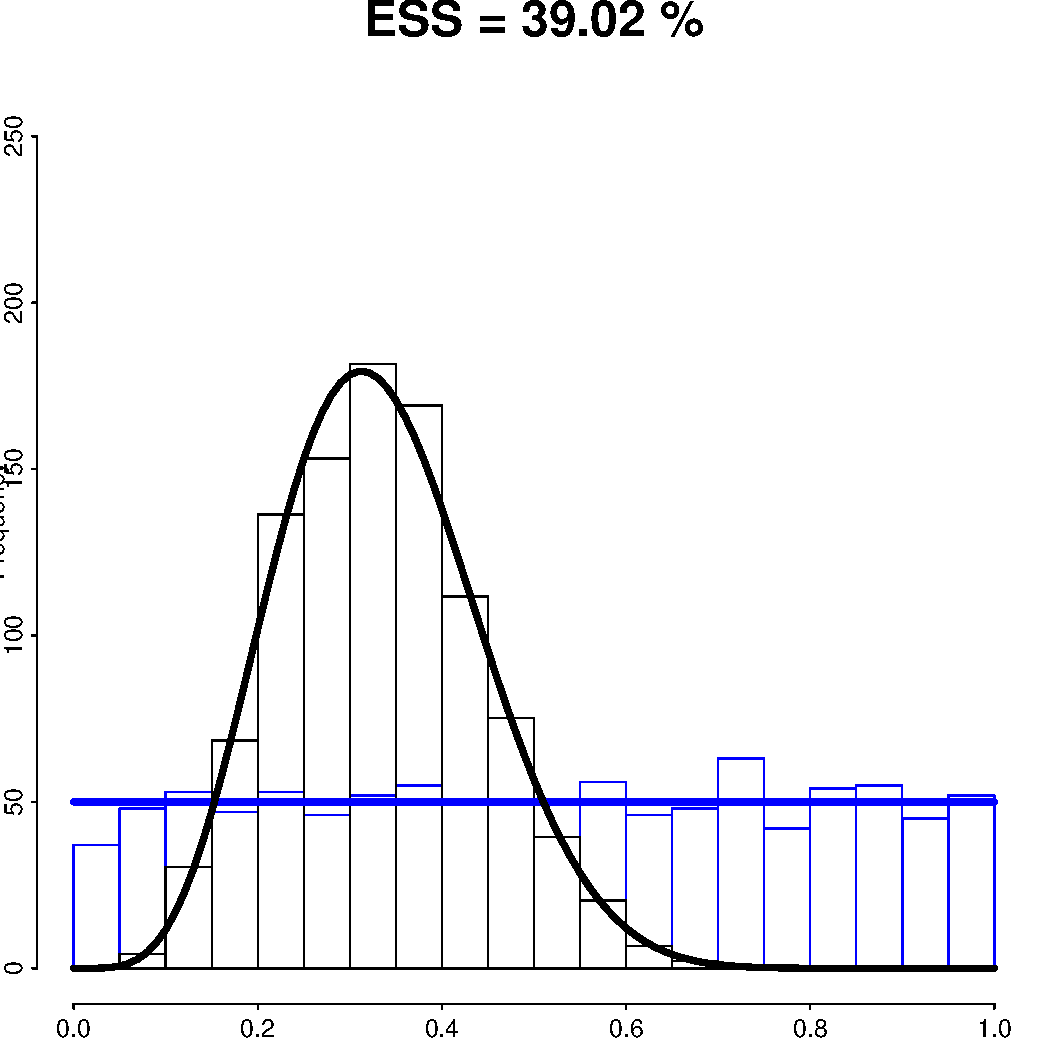
\includegraphics[height=.4\textheight]{../figs/ImportanceSampling-Beta-a06-b012-a1-b1-seed4} 
%     \end{tabular}
%     & 
%     \begin{tabular}{c}
%     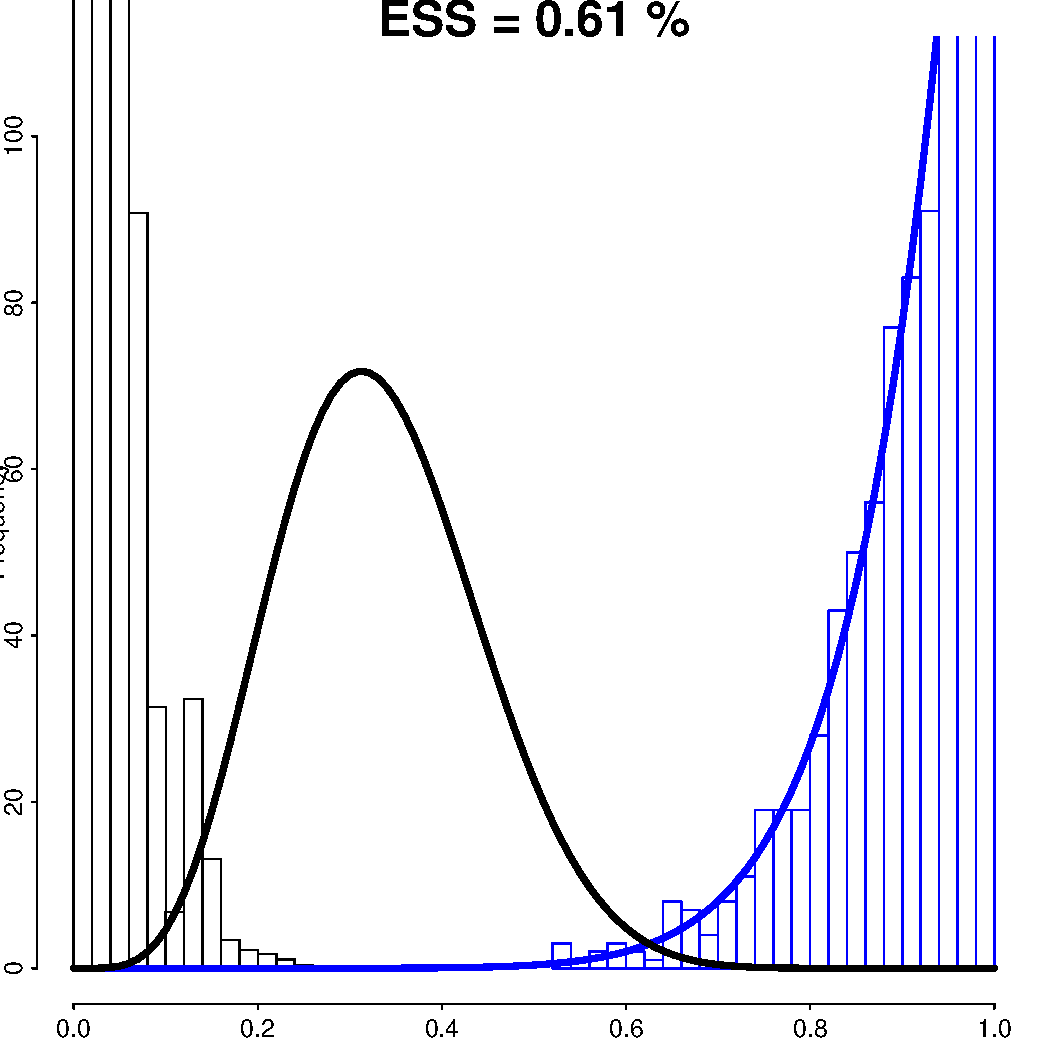
\includegraphics[height=.4\textheight]{../figs/ImportanceSampling-Beta-a06-b012-a10-b1-seed4} 
%     \end{tabular}
%     \\ \\
%     \begin{tabular}{c}
%     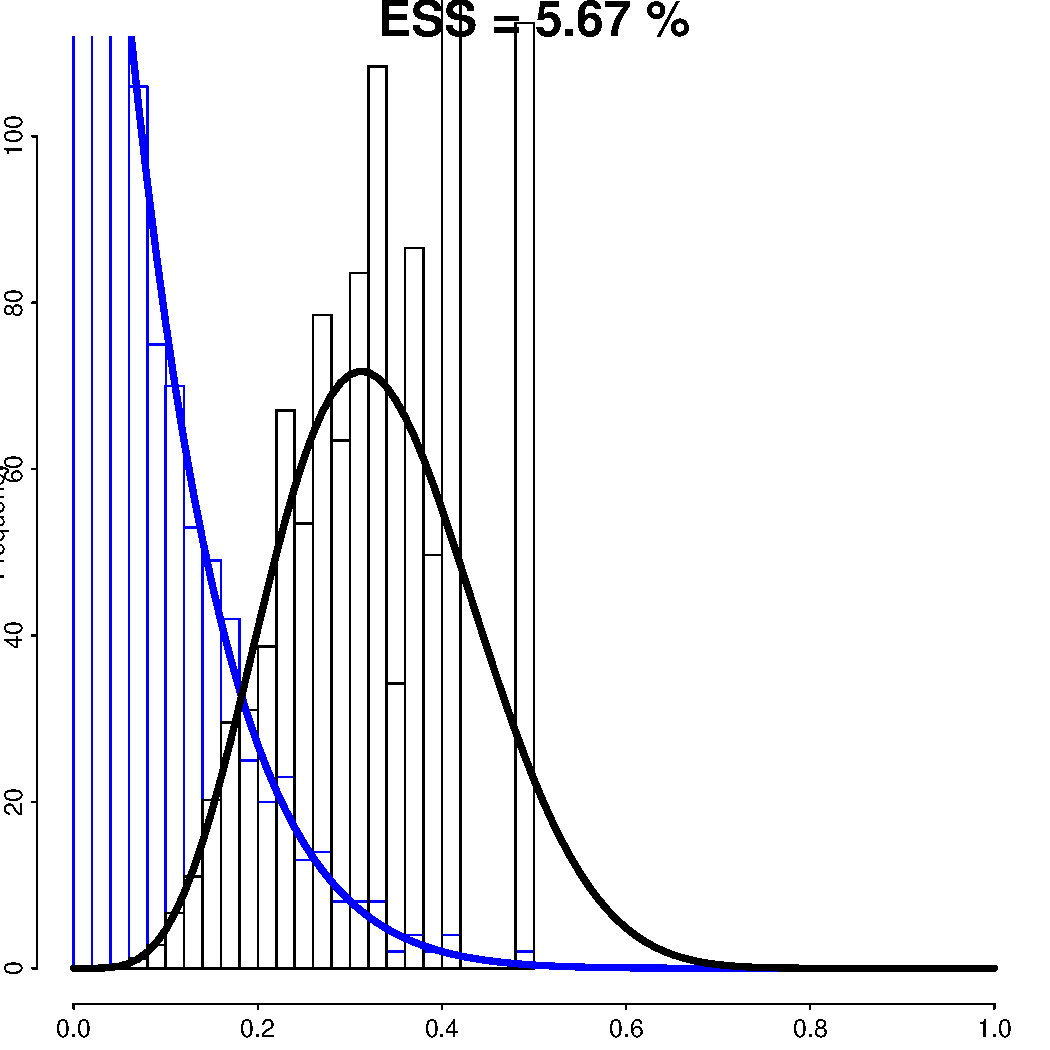
\includegraphics[height=.4\textheight]{../figs/ImportanceSampling-Beta-a06-b012-a1-b10-seed4} 
%     \end{tabular}
%     & 
%     \begin{tabular}{c}
%     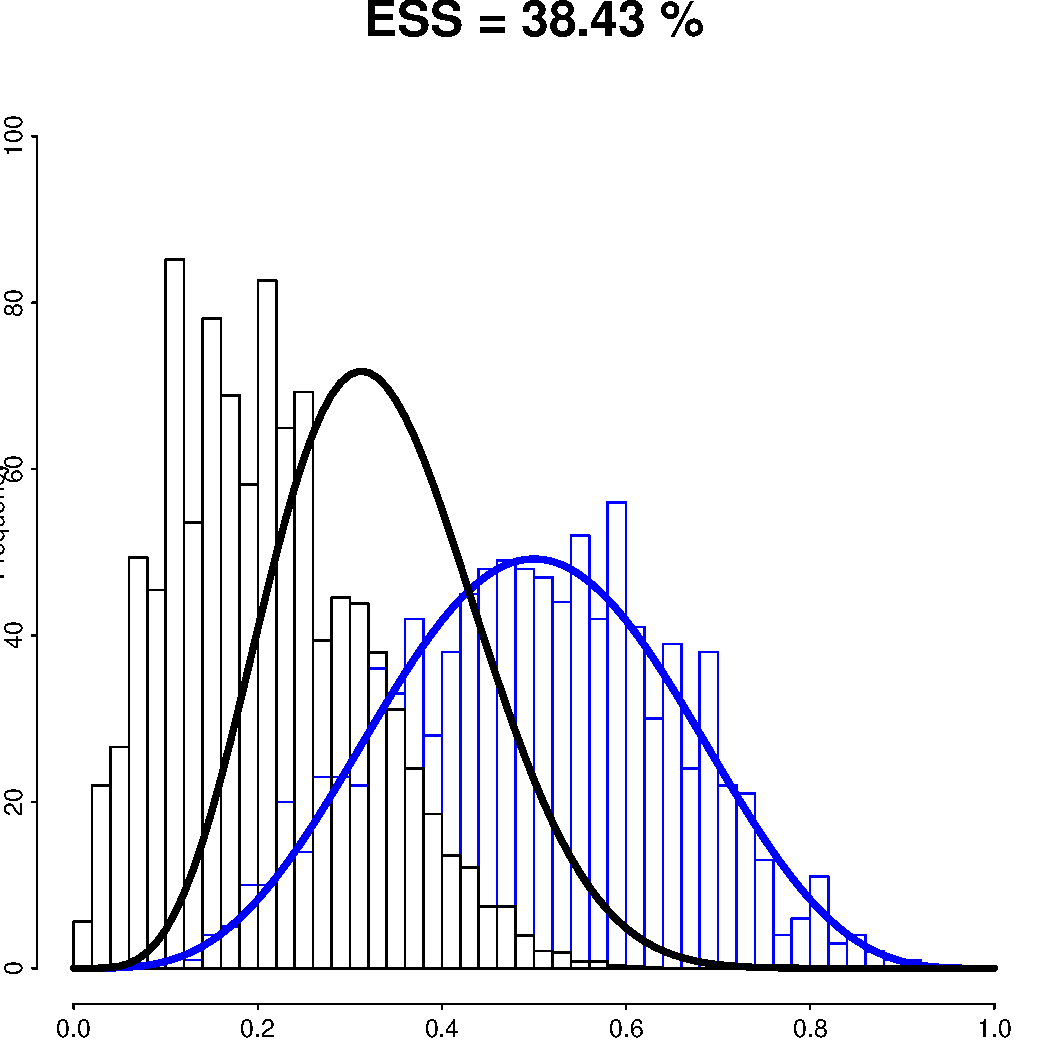
\includegraphics[height=.4\textheight]{../figs/ImportanceSampling-Beta-a06-b012-a5-b5-seed4} 
%     \end{tabular}
%   \end{tabular}
%   \end{center}
%  }  
% 
% %===================================================================
% \frame{ \frametitle{Importance of the proposal: another draw}

  \begin{center}
  \begin{tabular}{cc}
    \begin{tabular}{c}
    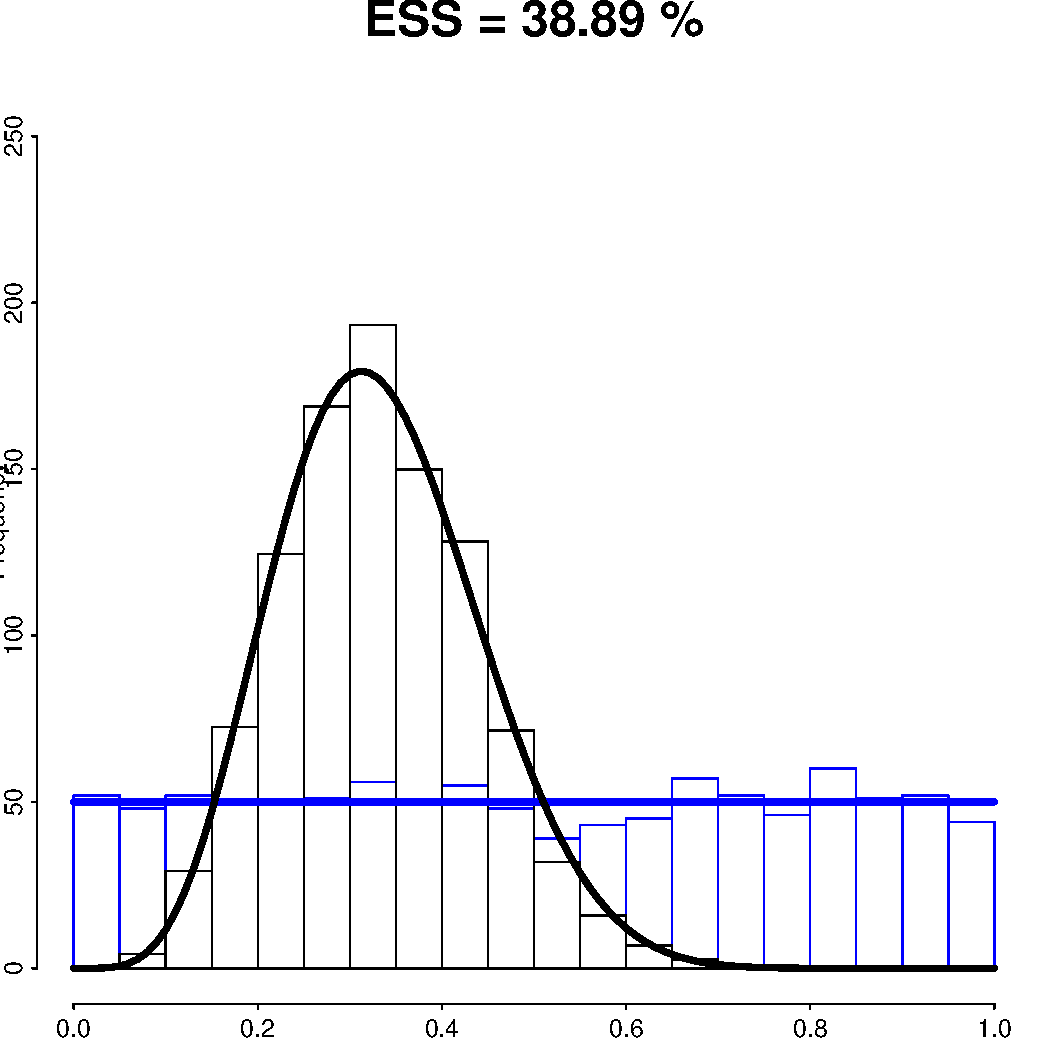
\includegraphics[height=.4\textheight]{../figs/ImportanceSampling-Beta-a06-b012-a1-b1-seed3} 
    \end{tabular}
    & 
    \begin{tabular}{c}
    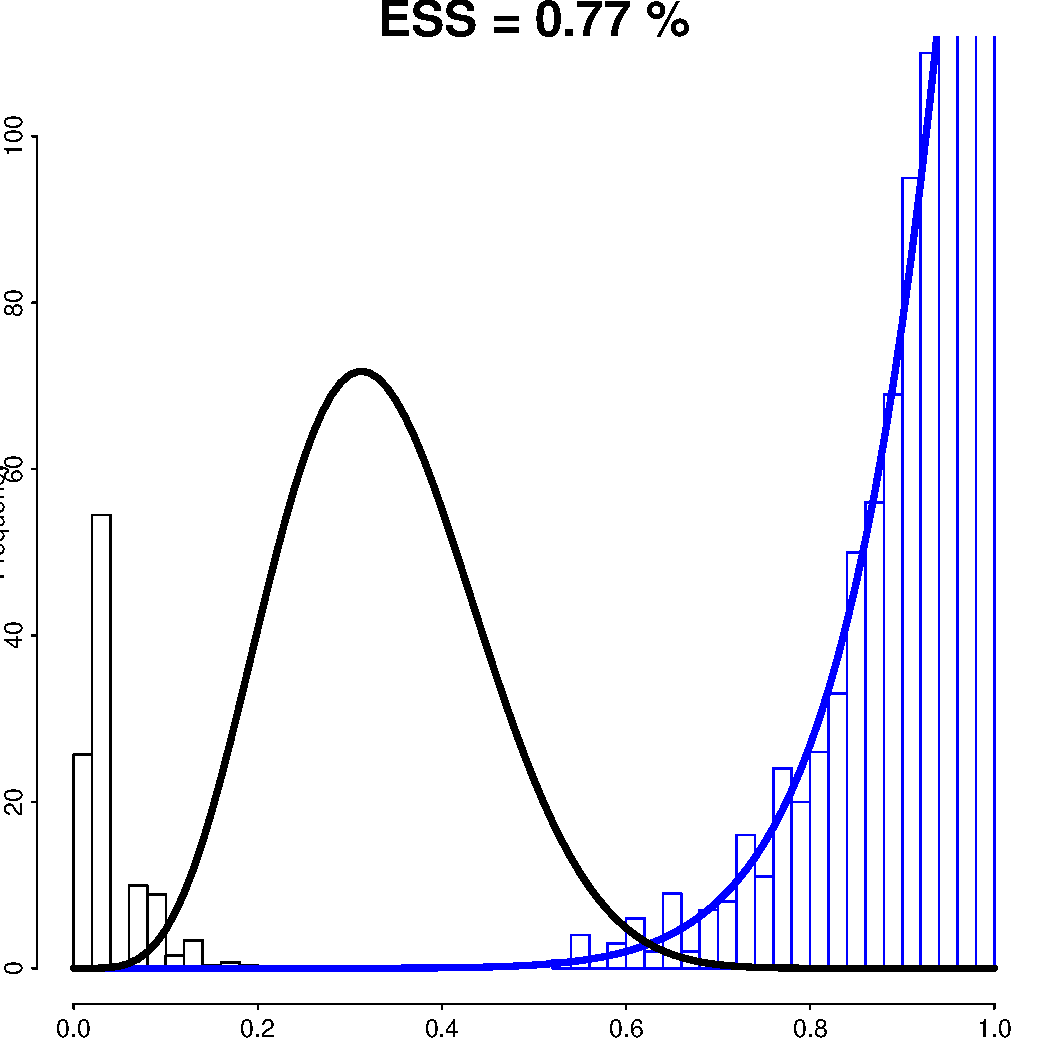
\includegraphics[height=.4\textheight]{../figs/ImportanceSampling-Beta-a06-b012-a10-b1-seed3} 
    \end{tabular}
    \\ \\
    \begin{tabular}{c}
    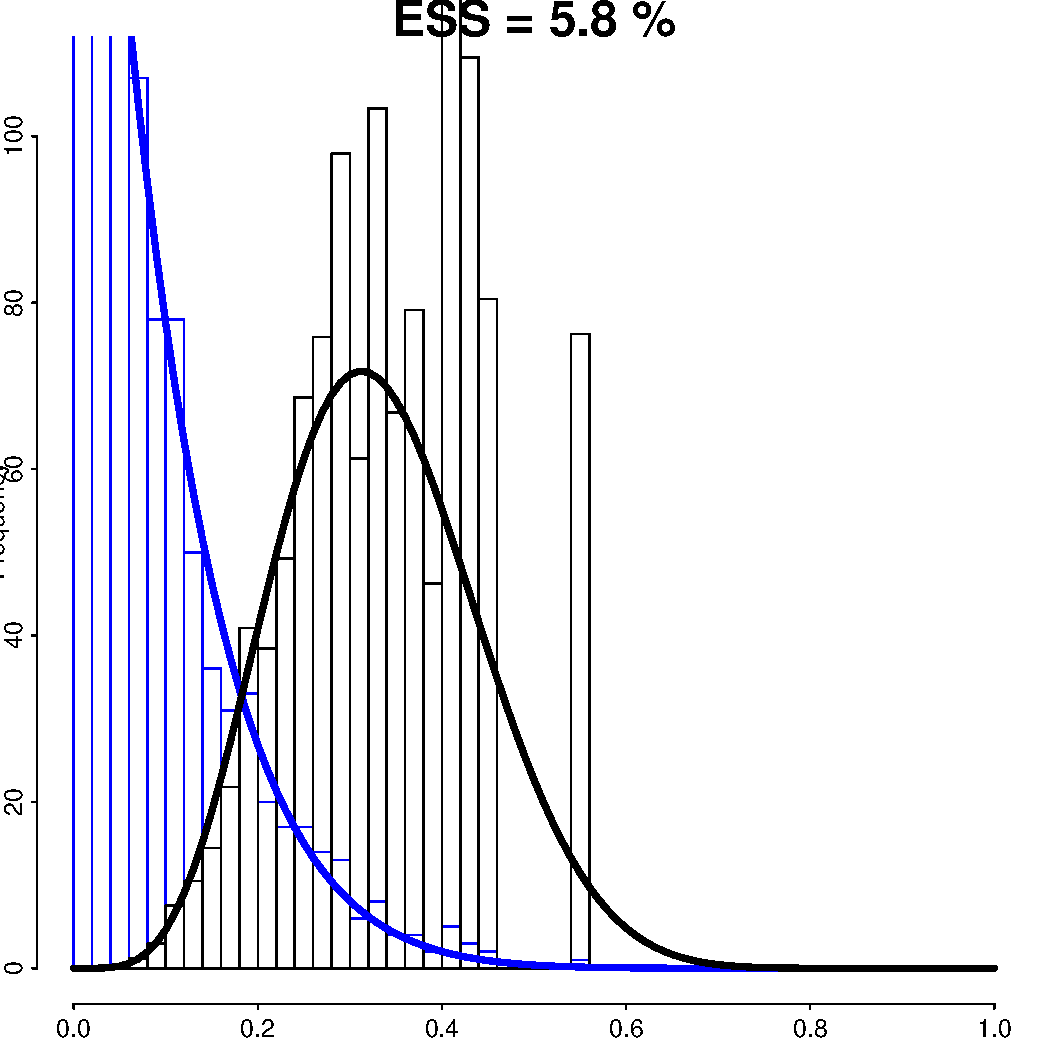
\includegraphics[height=.4\textheight]{../figs/ImportanceSampling-Beta-a06-b012-a1-b10-seed3} 
    \end{tabular}
    & 
    \begin{tabular}{c}
    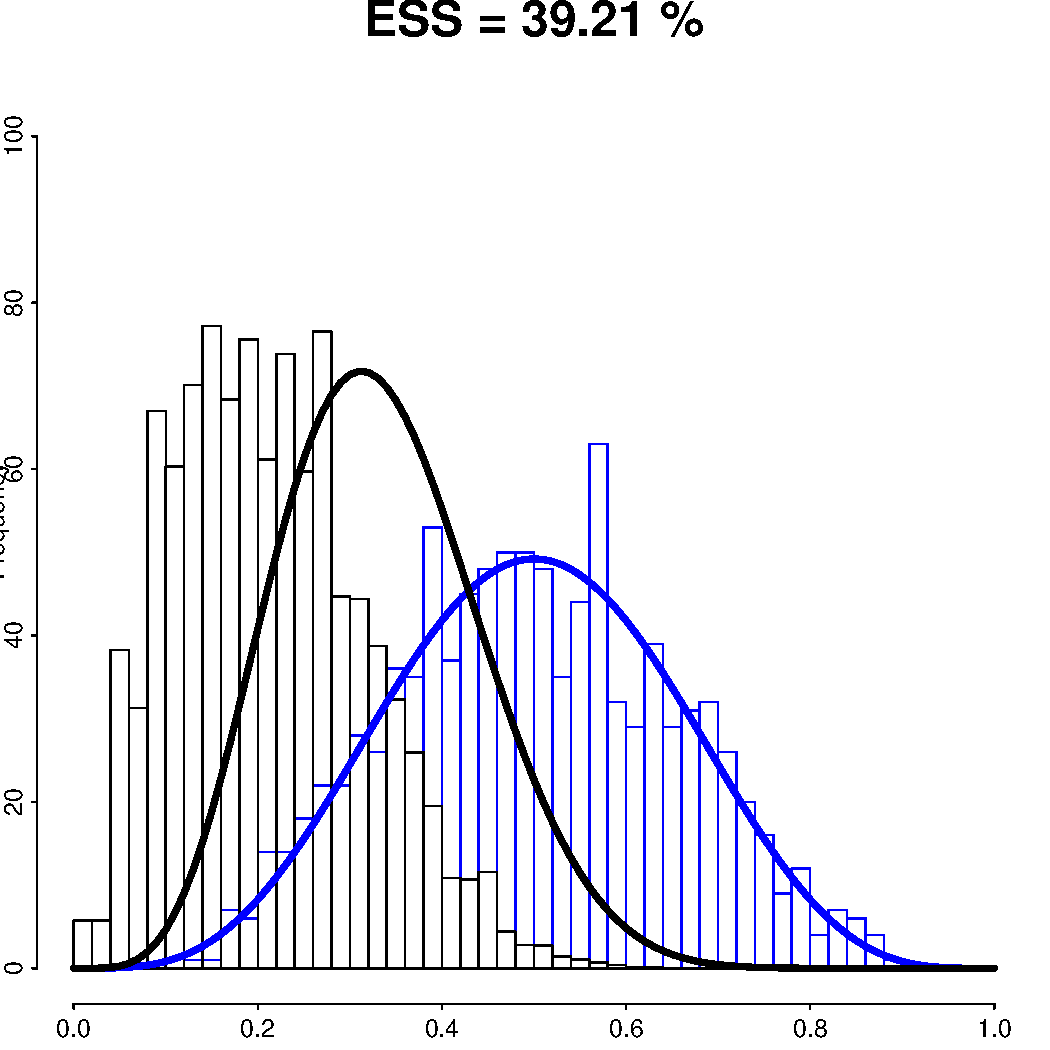
\includegraphics[height=.4\textheight]{../figs/ImportanceSampling-Beta-a06-b012-a5-b5-seed3} 
    \end{tabular}
  \end{tabular}
  \end{center}
 }  

%===================================================================
\frame{ \frametitle{Importance of the proposal: another draw}

  \begin{center}
  \begin{tabular}{cc}
    \begin{tabular}{c}
    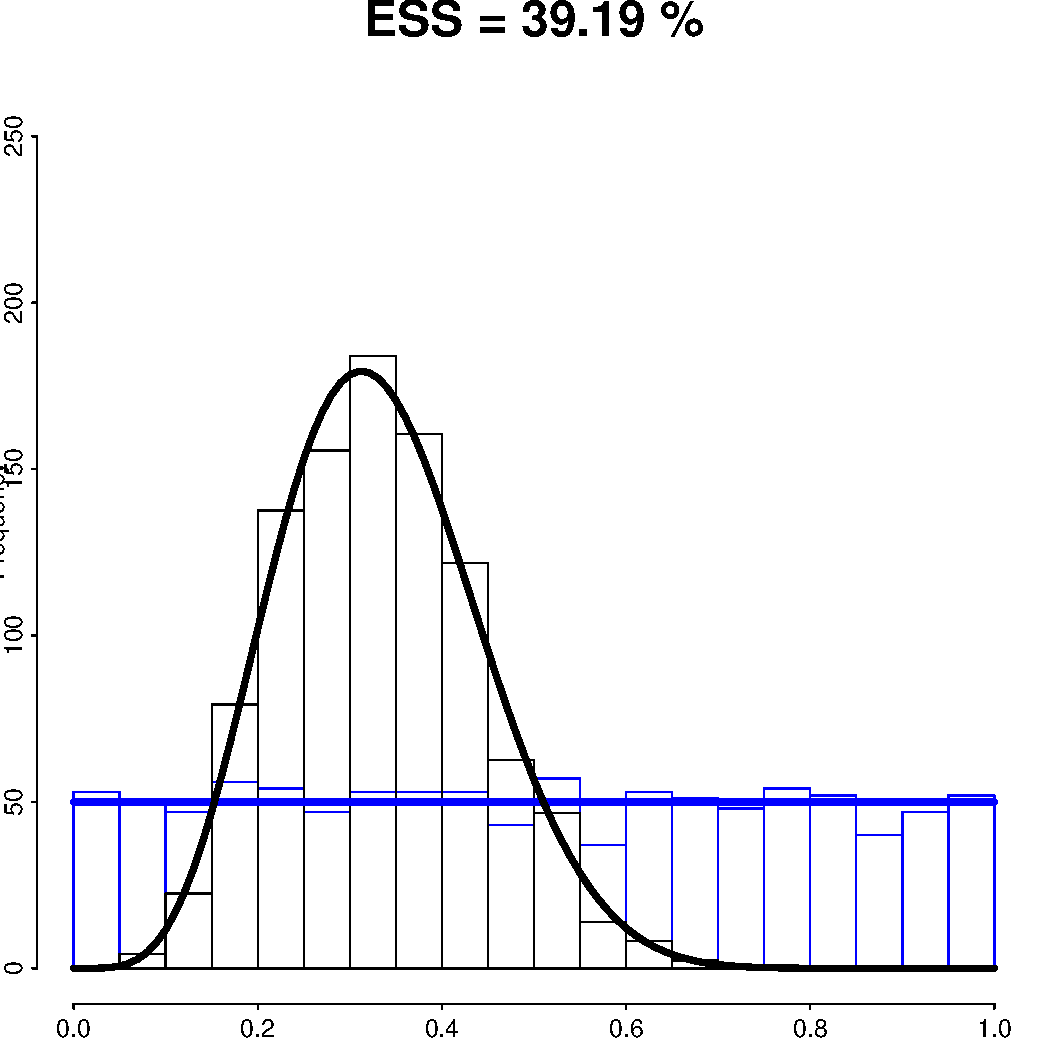
\includegraphics[height=.4\textheight]{../figs/ImportanceSampling-Beta-a06-b012-a1-b1-seed5} 
    \end{tabular}
    & 
    \begin{tabular}{c}
    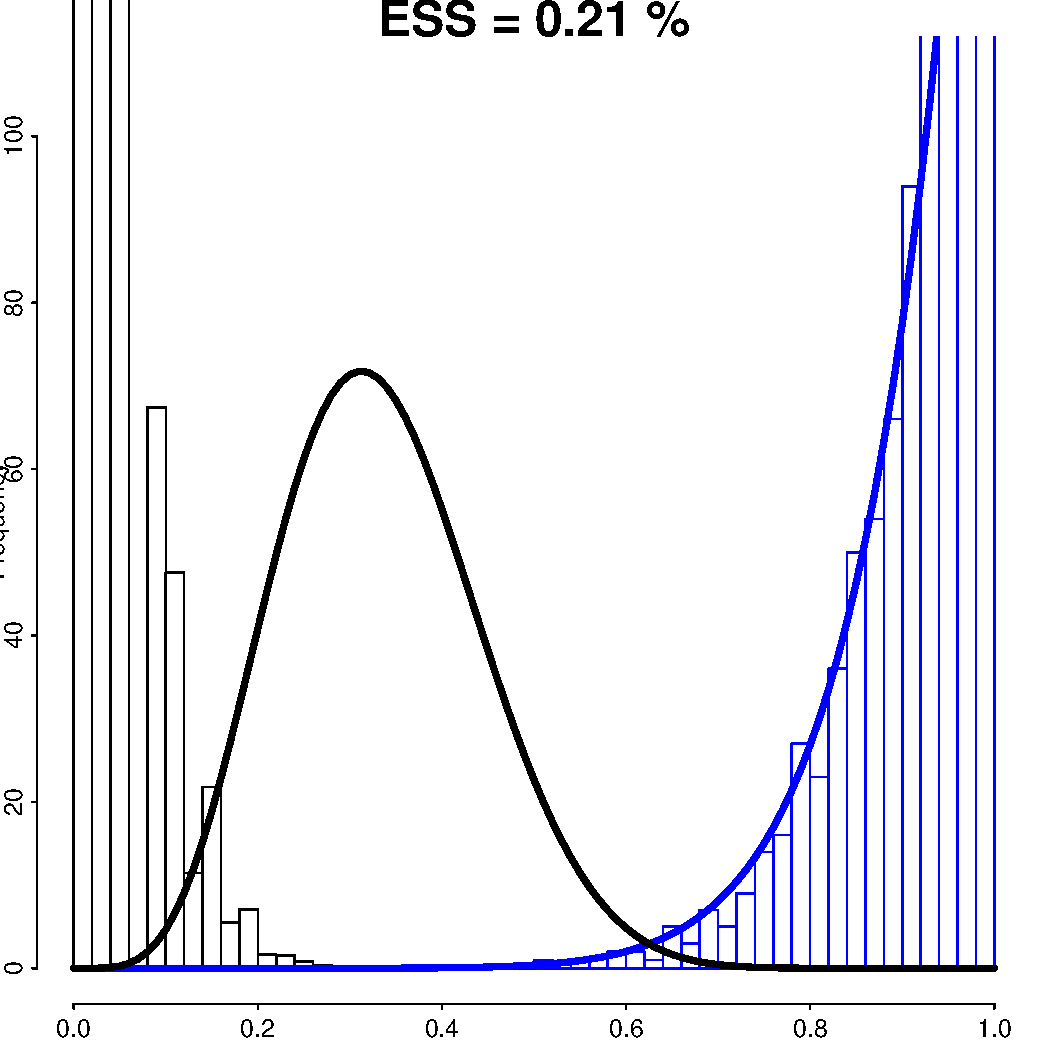
\includegraphics[height=.4\textheight]{../figs/ImportanceSampling-Beta-a06-b012-a10-b1-seed5} 
    \end{tabular}
    \\ \\
    \begin{tabular}{c}
    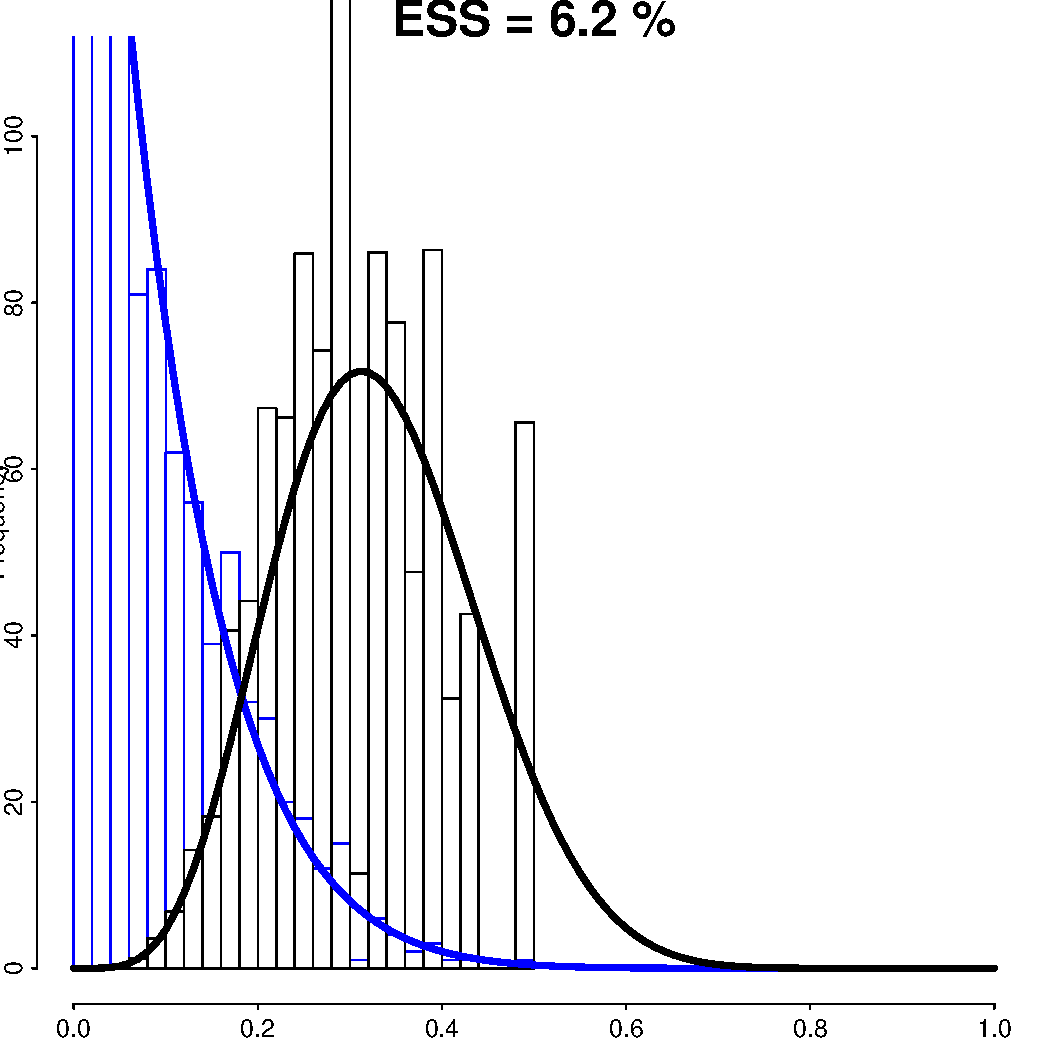
\includegraphics[height=.4\textheight]{../figs/ImportanceSampling-Beta-a06-b012-a1-b10-seed5} 
    \end{tabular}
    & 
    \begin{tabular}{c}
    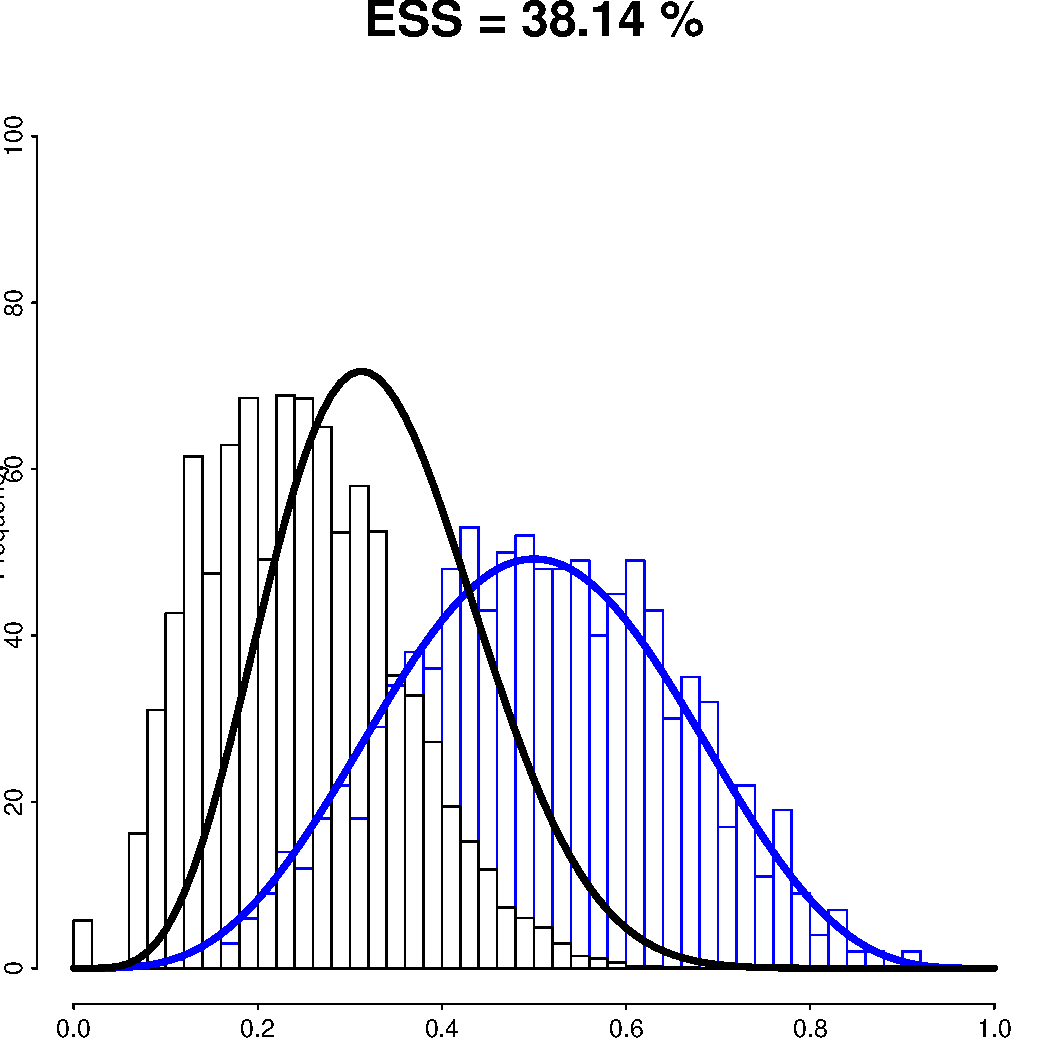
\includegraphics[height=.4\textheight]{../figs/ImportanceSampling-Beta-a06-b012-a5-b5-seed5} 
    \end{tabular}
  \end{tabular}
  \end{center}
 }  

% %===================================================================
% \frame{ \frametitle{Importance of the proposal: another draw}
% 
%   \begin{center}
%   \begin{tabular}{cc}
%     \begin{tabular}{c}
%     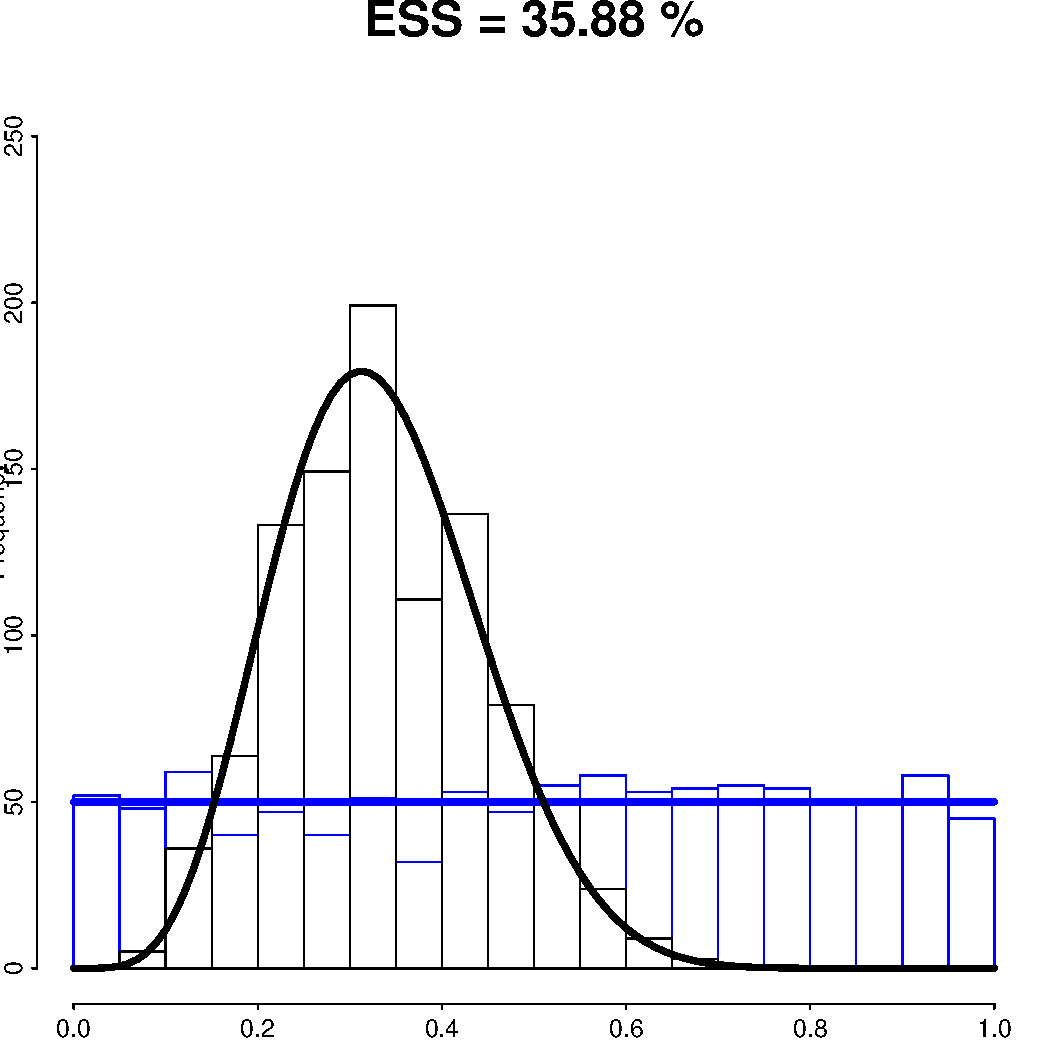
\includegraphics[height=.4\textheight]{../figs/ImportanceSampling-Beta-a06-b012-a1-b1-seed6} 
%     \end{tabular}
%     & 
%     \begin{tabular}{c}
%     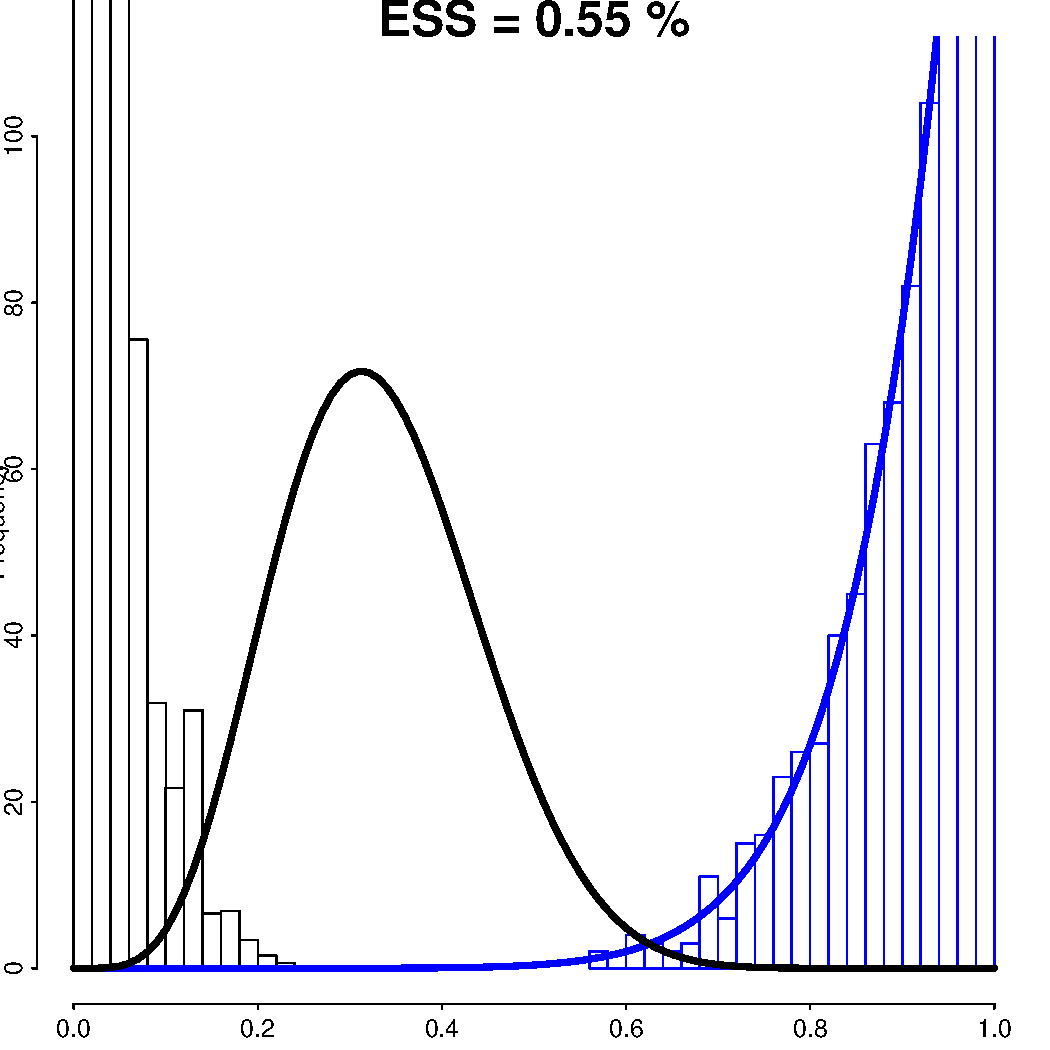
\includegraphics[height=.4\textheight]{../figs/ImportanceSampling-Beta-a06-b012-a10-b1-seed6} 
%     \end{tabular}
%     \\ \\
%     \begin{tabular}{c}
%     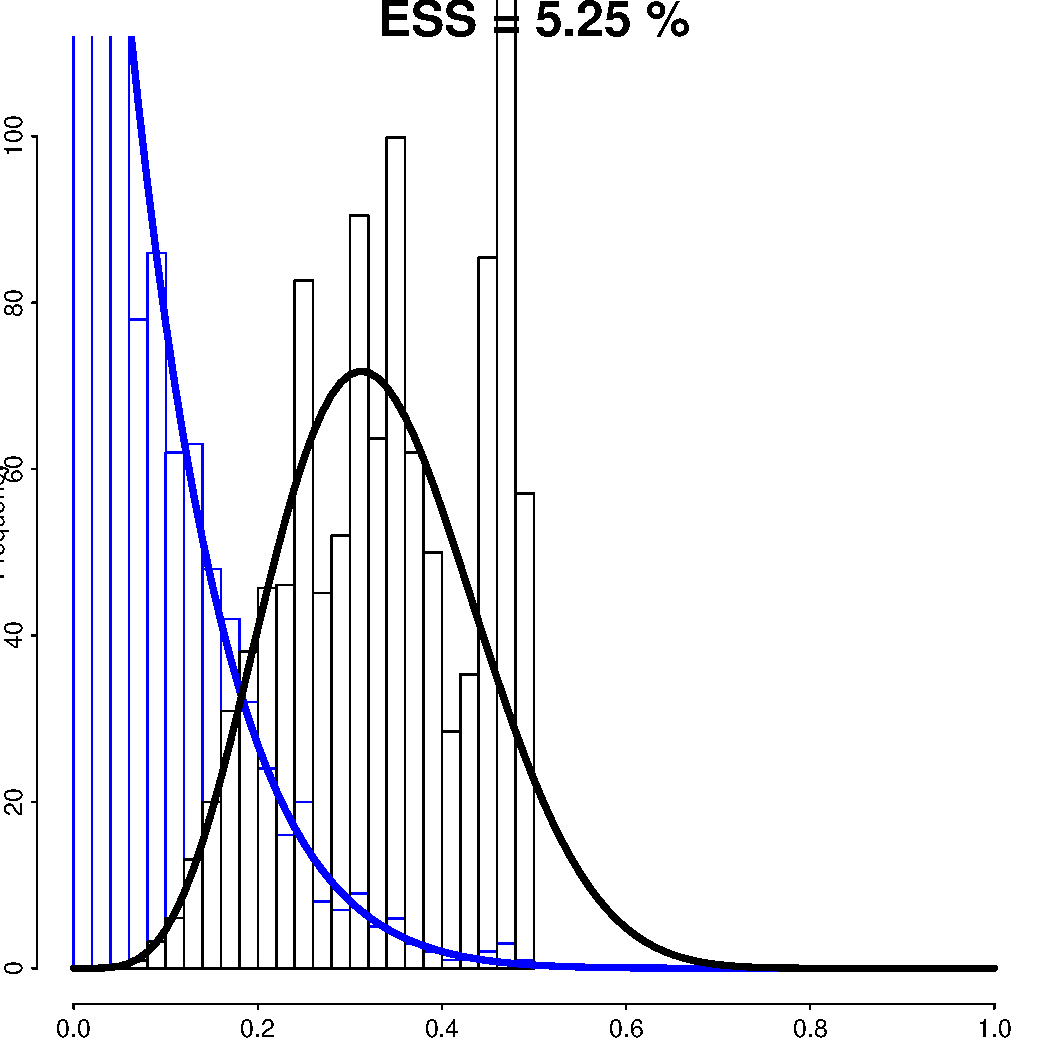
\includegraphics[height=.4\textheight]{../figs/ImportanceSampling-Beta-a06-b012-a1-b10-seed6} 
%     \end{tabular}
%     & 
%     \begin{tabular}{c}
%     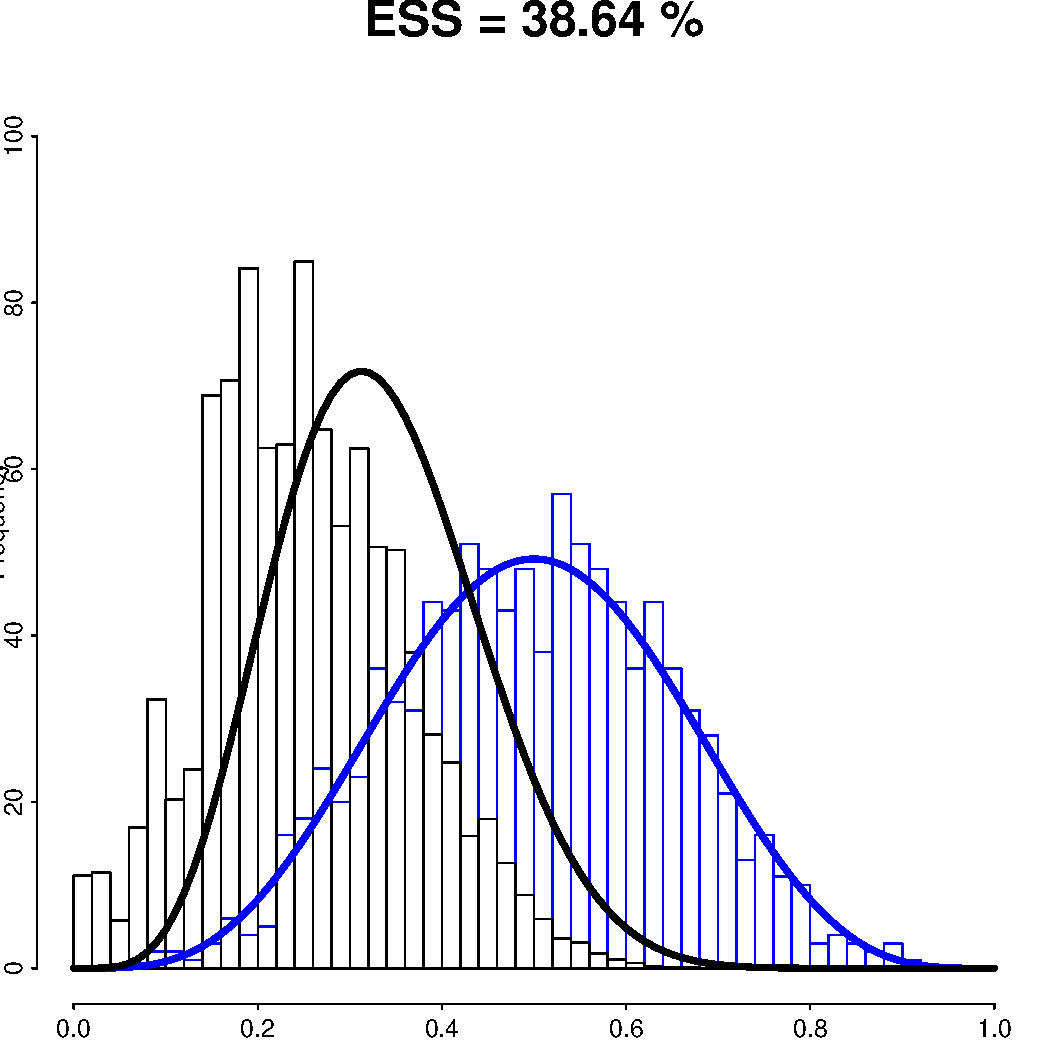
\includegraphics[height=.4\textheight]{../figs/ImportanceSampling-Beta-a06-b012-a5-b5-seed6} 
%     \end{tabular}
%   \end{tabular}
%   \end{center}
%  }  
% 
%===================================================================
\frame{ \frametitle{IS for posterior sampling}

  To evaluate $\Esp[f(\thetabf) | \Ybf]$, write it as
  \begin{align*}
    \Esp[f(\thetabf) \gv \Ybf] 
    = & \left. \int f(\thetabf) p(\thetabf, \Ybf) \d \thetabf \right/ p(\Ybf) 
    \; = \; \dots \\
%     = & \left. \int f(\thetabf) \pi(\thetabf) \ell(\Ybf \gv \thetabf) \d \thetabf \right/ \int \pi(\thetabf) \ell(\Ybf \gv \thetabf)  \d \thetabf \\
    = & \left. \int f(\thetabf) \frac{\pi(\thetabf) p(\thetabf \gv \Ybf)}{q(\thetabf)} q(\thetabf) \d \thetabf \right/ \int \frac{\pi(\thetabf) p(\thetabf \gv \Ybf)}{q(\thetabf)} q(\thetabf) \d \thetabf
  \end{align*}
  \begin{enumerate}
   \item sample
   $$
   (\thetabf^1, \dots, \thetabf^B) \text{ iid } \sim q
   $$
   \item compute the weights
   $$
   W(\thetabf^b) = \pi(\thetabf^b) p(\thetabf^b \gv \Ybf) \left/ q(\thetabf^b) \right.
   $$
   \item get
   $$
   \widehat{\Esp}[f(\thetabf) \gv \Ybf] = \sum_b W(\thetabf^b) f(\thetabf^b) \left/ \sum_b W(\thetabf^b)  \right.
   $$
   (slightly \emphase{biased}).
  \end{enumerate}
}

%===================================================================
\frame{ \frametitle{Good proposals}

  Choosing $q$ is critical

  \bigskip \pause
  \paragraph{Typical choices}
  \begin{itemize}
   \item Prior
   $$q(\thetabf) = \pi(\thetabf)$$
   \ra {far from the target $p(\thetabf \gv \Ybf)$: small $ESS$} \\ ~
   \item \pause MLE: 
   $$q(\thetabf) = \Ncal(\widehat{\thetabf}_{MLE}, \Var_\infty(\widehat{\thetabf}_{MLE}))$$  
   \ra {fine, as long as MLE is available} \\ ~
   \item \pause Variational Bayes, expectation propagation, ...: 
   $$
   q(\thetabf) = \arg\min_{q \in \Qcal} KL\left[q(\thetabf) \,||\, p(\thetabf \gv \Ybf\right]
   $$
   \ra fast and reasonably accurate
  \end{itemize}
}

%===================================================================
\frame{ \frametitle{Variational Bayes \& ML as a prior}

  \textcolor{blue}{prior}, \textcolor{red}{VB}, \textcolor{green}{MLE}, posterior 
  $$
  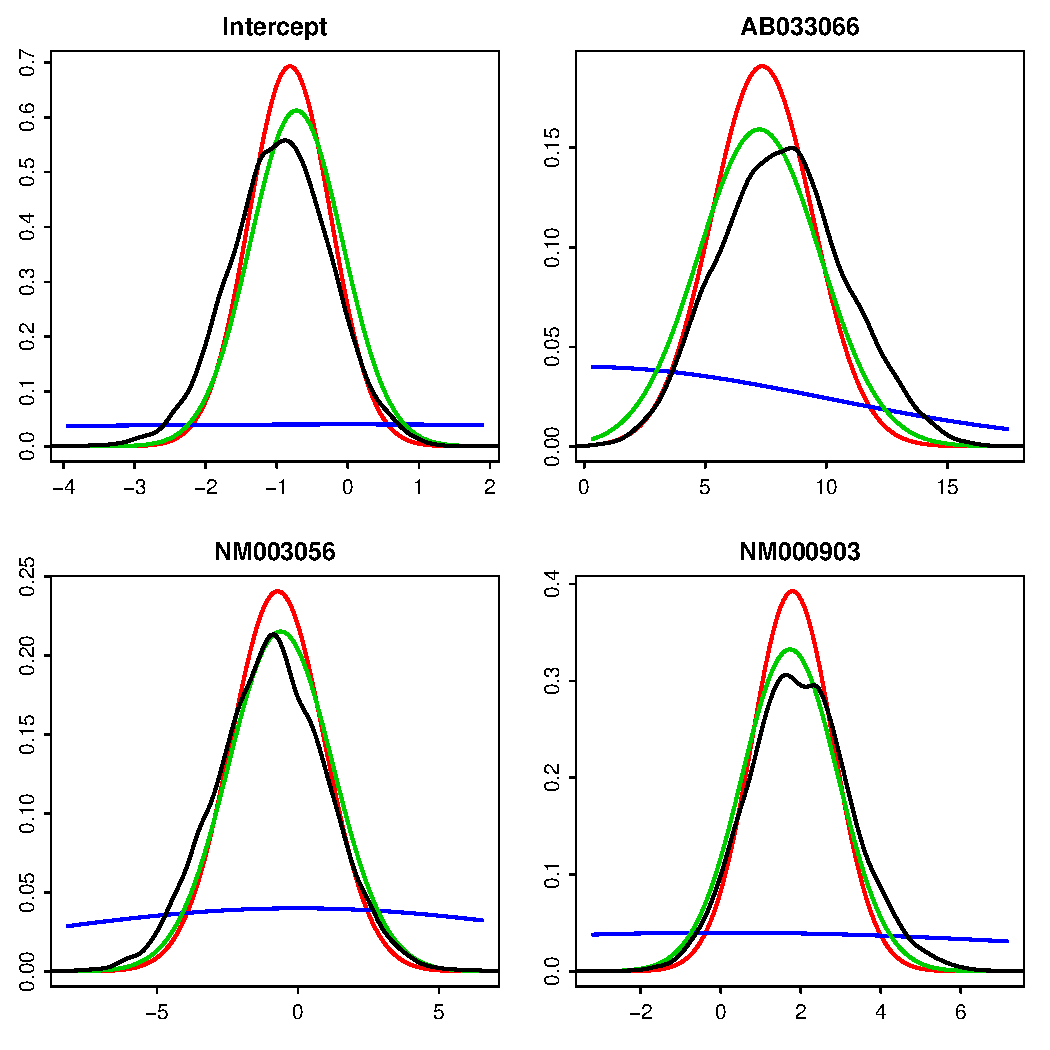
\includegraphics[width=.8\textwidth, height=.8\textheight]{\figfig/ISproposal-density}
  $$
}

%===================================================================
\frame{ \frametitle{Variational Bayes as a prior: joint distribution}

  \textcolor{red}{VB}, posterior 
  $$
  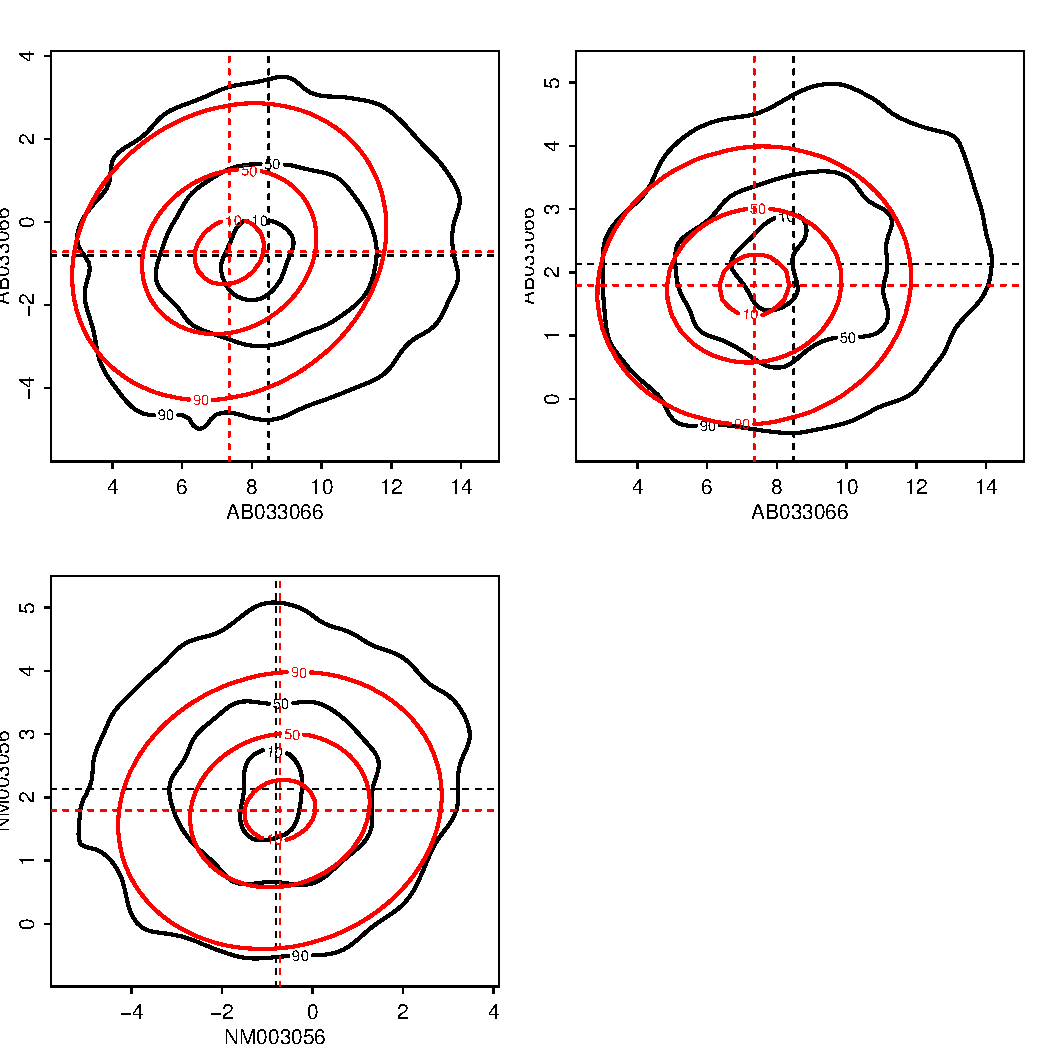
\includegraphics[width=.8\textwidth, height=.8\textheight]{\figfig/ISproposal-density2D}
  $$
}

%====================================================================
\subsection{Monte Carlo Markov chains (MCMC)}
\frame{\frametitle{Outline} \tableofcontents[currentsubsection]}
%====================================================================
\frame{ \frametitle{Limit distribution of Markov chain}

  \paragraph{Definition.} Let $\{\phibf^b\}_{b \geq 0}$ be a Markov chain with
  \begin{itemize}
   \item initial distribution $\phibf^0 \sim \nu$,
   \item transition kernel $\phibf^b \gv \phibf^{b-1} \sim \kappa(\cdot \gv \phibf^{b-1})$:
  \end{itemize}
%   $$
%   p\left(\{\phibf^b\} \right) = \nu(\phibf^0) \times \kappa(\phibf^1 \gv \phibf^0) \times \kappa(\phibf^2 \gv \phibf^1) \times \kappa(\phibf^3 \gv \phibf^2) \times \dots
% %   \prod_{b\geq 1} \kappa(\phibf^b \gv \phibf^{b-1})
%   $$
  $\{\phibf^b\}_{b \geq 0}$ is said to be {\sl ergodic} if
  \begin{itemize}
   \item it admits a \emphase{unique stationary distribution} $\mu$:
   $$
   \phibf^{b-1} \sim \mu \qquad \Rightarrow \qquad \phibf^b \sim \mu
   $$
   \item for \emphase{any initial distribution} $\nu$, $\phibf^b$ converges towards $\mu$ in distribution
   $$
   \phibf^b \overset{\Delta}{\underset{b \rightarrow \infty}{\longrightarrow}} \mu
   $$
  \end{itemize}
  
  \bigskip
  \paragraph{Ergodicity conditions.}
  \begin{itemize}
   \item Finite state space: irreducibility, aperiodicity
   \item Infinite state space: the same + positive recurrence
  \end{itemize}
}

%====================================================================
\frame{ \frametitle{Use for Bayesian inference}

  \paragraph{Aim.} Sample from
  $$
  p(\thetabf \gv \Ybf)
  $$
  
  \bigskip \bigskip 
  \paragraph{Idea.} 
  \begin{itemize}
   \item Construct an ergodic Markov chain $\{\thetabf^b\}_{b \geq 0}$ with stationary distribution
   $$
   \mu(\thetabf) = p(\thetabf \gv \Ybf)
   $$
   \item Choose 'any' initial $\nu$ and simulate $\{\thetabf^b\}_{b \geq 0}$ \\ ~
   \item Until it 'reaches' its stationary distribution
  \end{itemize}
}

%====================================================================
\frame{ \frametitle{Metropolis-Hastings}

  \paragraph{Algorithm.} Define a shift kernel $\lambda(\cdot \gv \thetabf)$
  \begin{itemize}
   \item \pause Start with $\thetabf^0$
   \item \pause At step $b$, 
   \begin{enumerate}
    \item \pause sample $\thetabf' \sim \lambda(\cdot \gv \thetabf^{b-1})$;
   \item \pause compute the Metropolis-Hastings ratio (acceptance probability)
   $$
   \alpha(\thetabf', \thetabf^{b-1}) 
   = \frac{\lambda(\thetabf^{b-1} \gv \thetabf')}{\lambda(\thetabf' \gv \thetabf^{b-1})} \frac{p(\thetabf' \gv \Ybf)}{p(\thetabf^{b-1} \gv \Ybf)}
   \pause = \frac{\lambda(\thetabf^{b-1} \gv \thetabf')}{\lambda(\thetabf' \gv \thetabf^{b-1})} \frac{\pi(\thetabf') \ell(\Ybf \gv \thetabf')}{\pi(\thetabf^{b-1}) \ell(\Ybf \gv \thetabf^{b-1})};
   $$
   \item \pause $\text{set } \thetabf^b= \left\{
	 \begin{array}{ll}
	   \thetabf' & \text{with probability $\max(1, \alpha(\thetabf', \thetabf^{b-1}))$,} \\
	   \thetabf^{b-1} & \text{otherwise.}
	 \end{array} 
    \right.$
   \end{enumerate}
  \end{itemize}
  
  \bigskip \pause
  \paragraph{Properties.} 
  \begin{enumerate}
   \item $\lambda$ and $\alpha$ define a Markov chain with stationary distribution $\mu(\thetabf) = p(\thetabf \gv \Ybf)$.
   \item If $\lambda(\cdot \gv \thetabf)$ is symmetric, $\alpha$ reduce to ${\pi(\thetabf') \ell(\Ybf \gv \thetabf')}/ [{\pi(\thetabf^{b-1}) \ell(\Ybf \gv \thetabf^{b-1})}]$
  \end{enumerate}
}

%====================================================================
\frame{ \frametitle{Metropolis-Hastings for logistic regression}

  \paragraph{Model.} 
  \begin{align*}
   \thetabf & \sim \pi(\thetabf) = \Ncal(\Obf_p, 100 \, \Ibf_p)\\
   \Ybf \gv \thetabf & \sim \ell(\Ybf \gv \thetabf) 
   = \prod_i \left(\frac{e^{\xbf_i^\intercal \thetabf}}{1 + e^{\xbf_i^\intercal \thetabf}}\right)^{y_i} \left(\frac{e^{\xbf_i^\intercal \thetabf}}{1 + e^{\xbf_i^\intercal \thetabf}}\right)^{1-y_i}
  \end{align*}

  \bigskip \bigskip \pause
  \paragraph{Algorithm settings.} 
  $$\thetabf^0 = \Obf_p$$
  $$\lambda( \cdot \gv \thetabf) = \Ncal(\Obf_p, .5 \, \Ibf_p)$$
}

%====================================================================
\frame{ \frametitle{M-H for logistic regression: R code}

  \pause
  \footnotesize{\tt 
  mu.prior = rep(0, p); Sigma.prior = 100*diag(p); Sigma.shift = .5*diag(p) \\ \pause
  theta.sample = matrix(0, B, p); \\ \pause
  ~ \\
  theta.cur = theta.sample[1, ] \\ \pause
  logprior.cur = dmvnorm(theta.cur, mean=mu.prior, sigma=Sigma.prior, log=T) \\ \pause
  prob.cur = plogis(X\%*\%theta.cur) \\ \pause
  loglik.cur = sum(dbinom(Y, 1, prob.cur, log=T)) \\ \pause
  ~ \\
  for (b in 2:B)\{ \\ \pause
  \qquad theta.prop = rmvnorm(1, mean=theta.sample[b-1, ], sigma=Sigma.shift)[1, ] \\ \pause
  \qquad logprior.prop = dmvnorm(theta.prop, mean=mu.prior, sigma=Sigma.prior, log=T) \\ \pause
  \qquad prob.prop = plogis(X\%*\%theta.prop) \\ \pause
  \qquad loglik.prop = sum(dbinom(Y, 1, prob.prop, log=T)) \\ \pause
  ~ \\
  \qquad alpha = exp(logprior.prop + loglik.prop - logprior.cur - loglik.cur) \\ \pause
  \qquad if(runif(1) < alpha)\{ \\ 
  \qquad \qquad theta.sample[b, ] = theta.cur = theta.prop \\ 
  \qquad \qquad logprior.cur = logprior.prop; loglik.cur = loglik.prop \\ \pause
  \qquad \}else\{ \\
  \qquad \qquad theta.sample[b, ] = theta.sample[b-1, ] \\
  \qquad \} \\ \pause
  \} \\
  }
}

%====================================================================
\frame{ \frametitle{Sanity checks}

  \bigskip
  \paragraph{Setting.} Sample $1.2 \; 10^5$ $\thetabf$, remove first $2 \; 10^4$, extract every 10 \ra $B = 10^4$. \\ ~

  \begin{tabular}{cc}
    \begin{tabular}{p{.3\textwidth}}
	 \begin{itemize}
	 \item \onslide+<1->{Acceptance rate} \\ ~
	 \item \onslide+<2->{Stationarity: \\ 
	   var. shift = .1} 
	   \onslide+<3->{, .5} 
	   \onslide+<4->{, 1 \\ ~}
	 \item \onslide+<5->{Autocorrelation  
	   $\Cor(\theta_j^{b-1}, \theta_j^b)$: \\
	   var. shift = .1} 
	   \onslide+<6->{, .5} 
	   \onslide+<7->{, 1 \\ ~}
	 \item \onslide+<8->{And many others (e.g. Gelman-Rubin)}
	 \end{itemize}
	 \\~ \\~ \\~ \\~ \\~ \\~ \\~ \\~ 
    \end{tabular}
    & 
    \hspace{-.02\textwidth}
    \begin{tabular}{p{.7\textwidth}}
	 \begin{overprint}
	 %===================
	  \onslide<1>
	  \vspace{.3\textheight}
	  \begin{tabular}{lrrrr}
	   variance shift & 0.1  & 0.5  & 1 \\ 
	   \hline 
	   acceptance rate  & 0.421  & 0.125  & 0.053 
	   \end{tabular} 
	 %=================
	  \onslide<2>
	  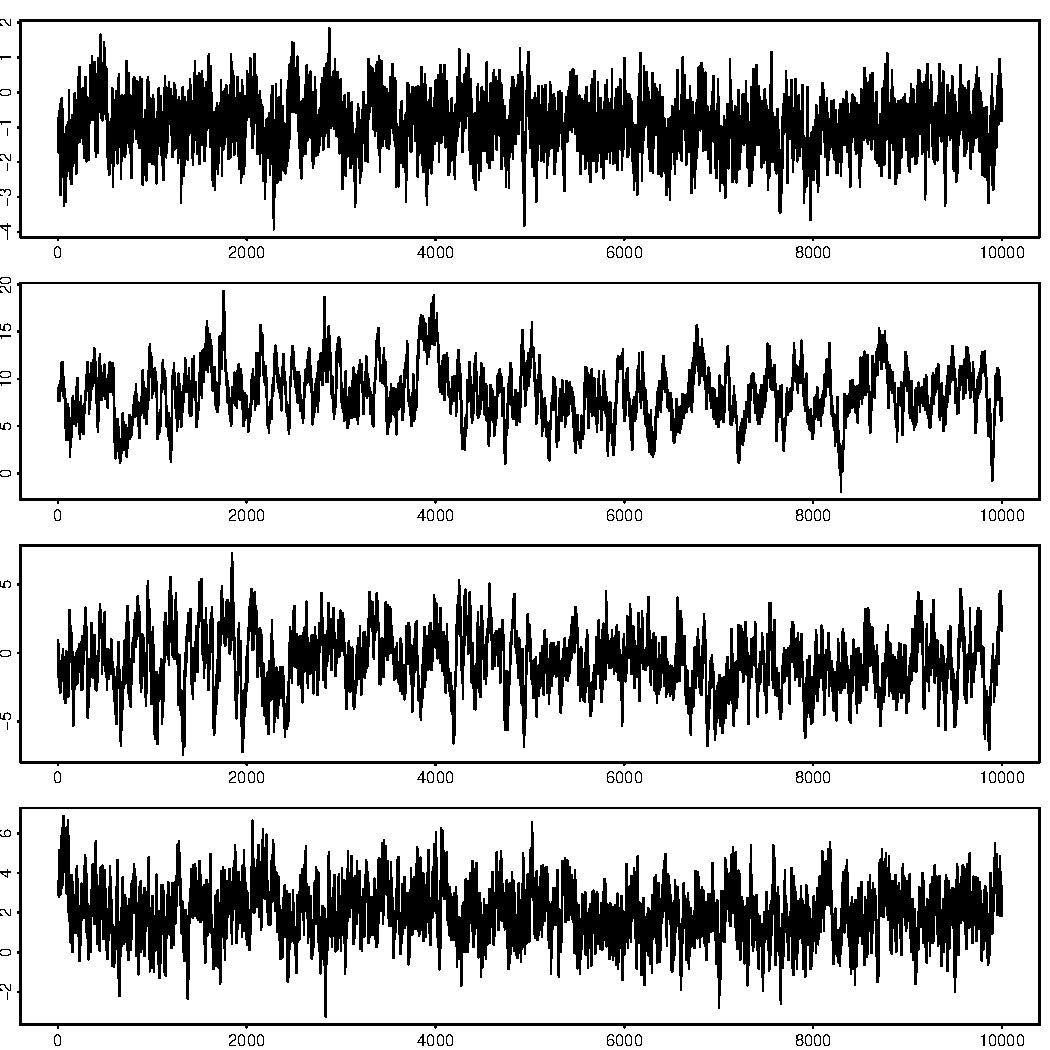
\includegraphics[width=.5\textwidth]{../figs/MH-path-10shift1}
	 %=================
	  \onslide<3>
	  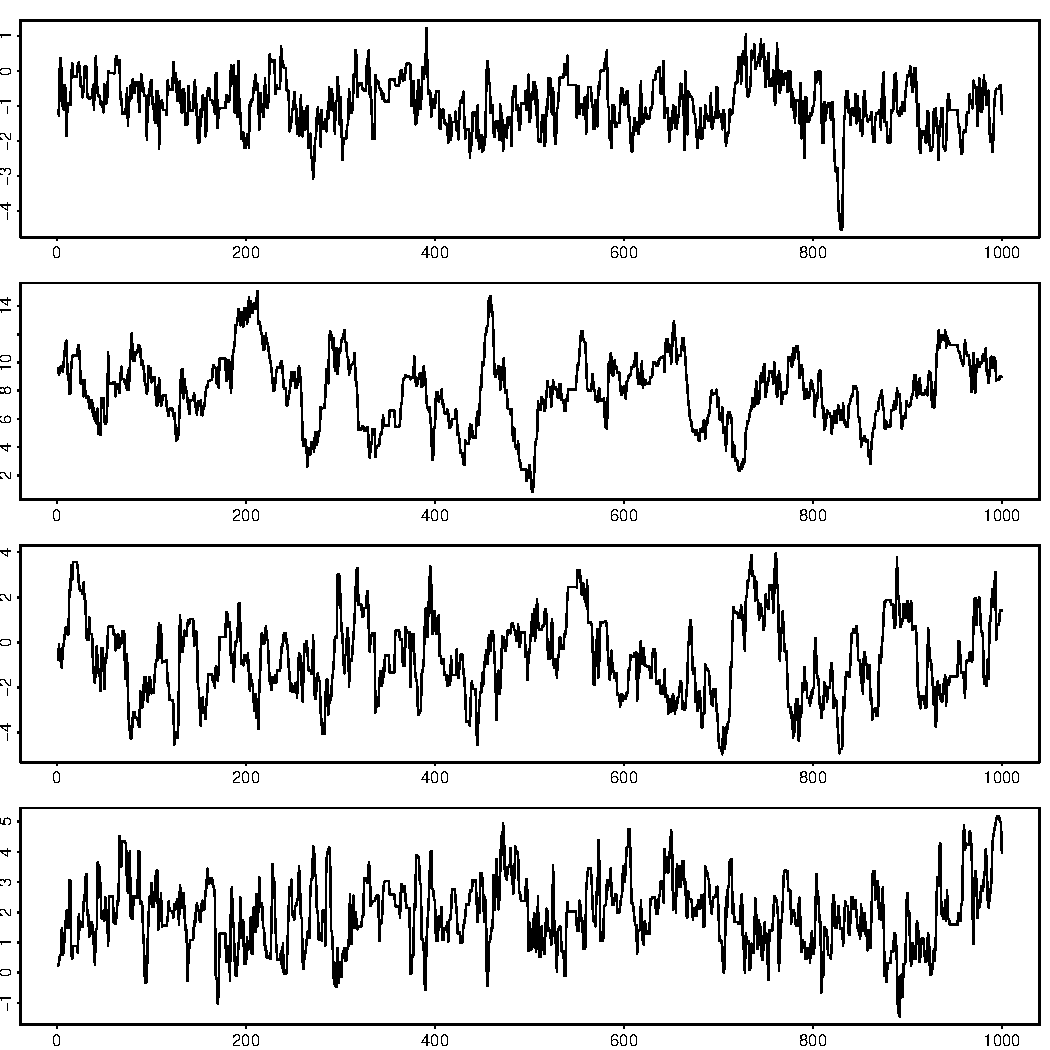
\includegraphics[width=.5\textwidth]{../figs/MH-path-10shift5}
	 %=================
	  \onslide<4>
	  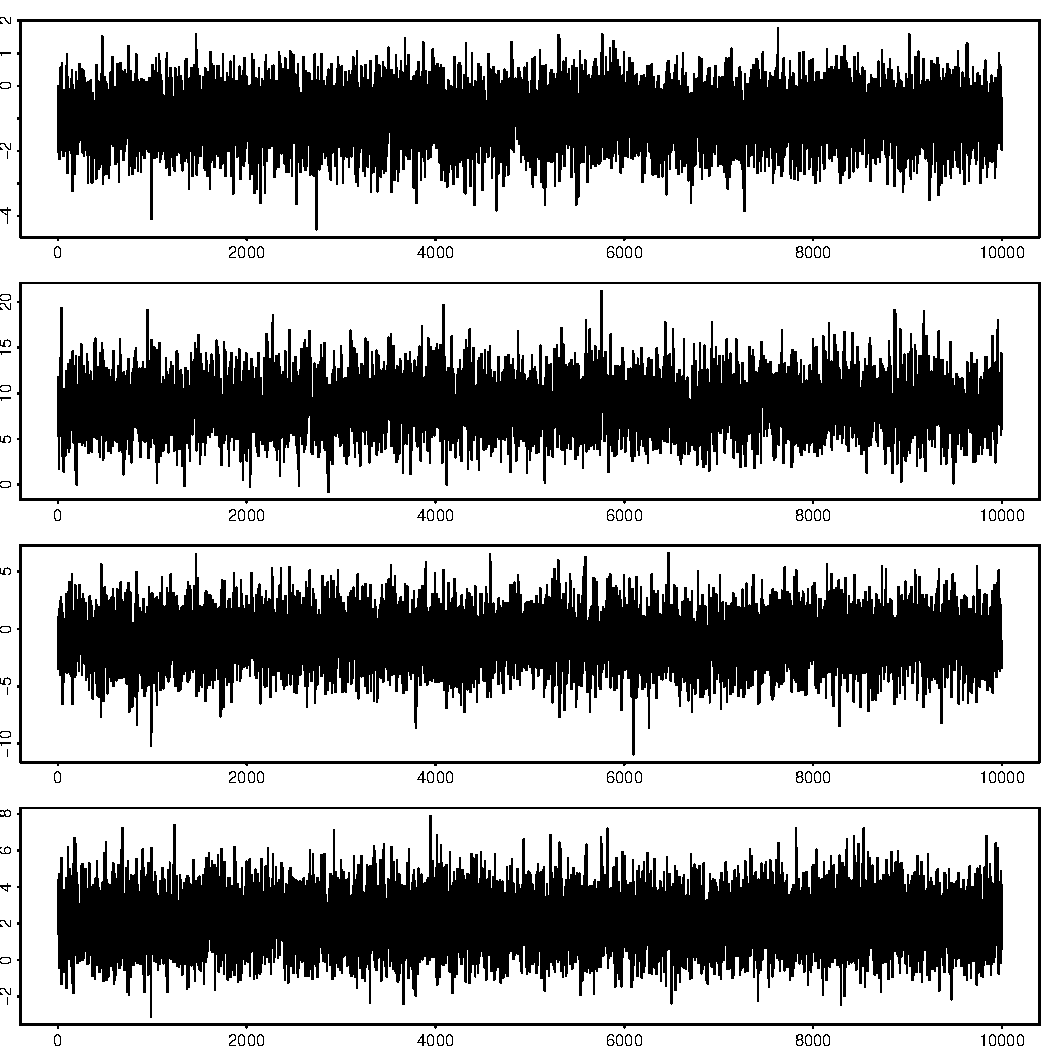
\includegraphics[width=.5\textwidth]{../figs/MH-path-10shift10}
	 %=================
	  \onslide<5>
	  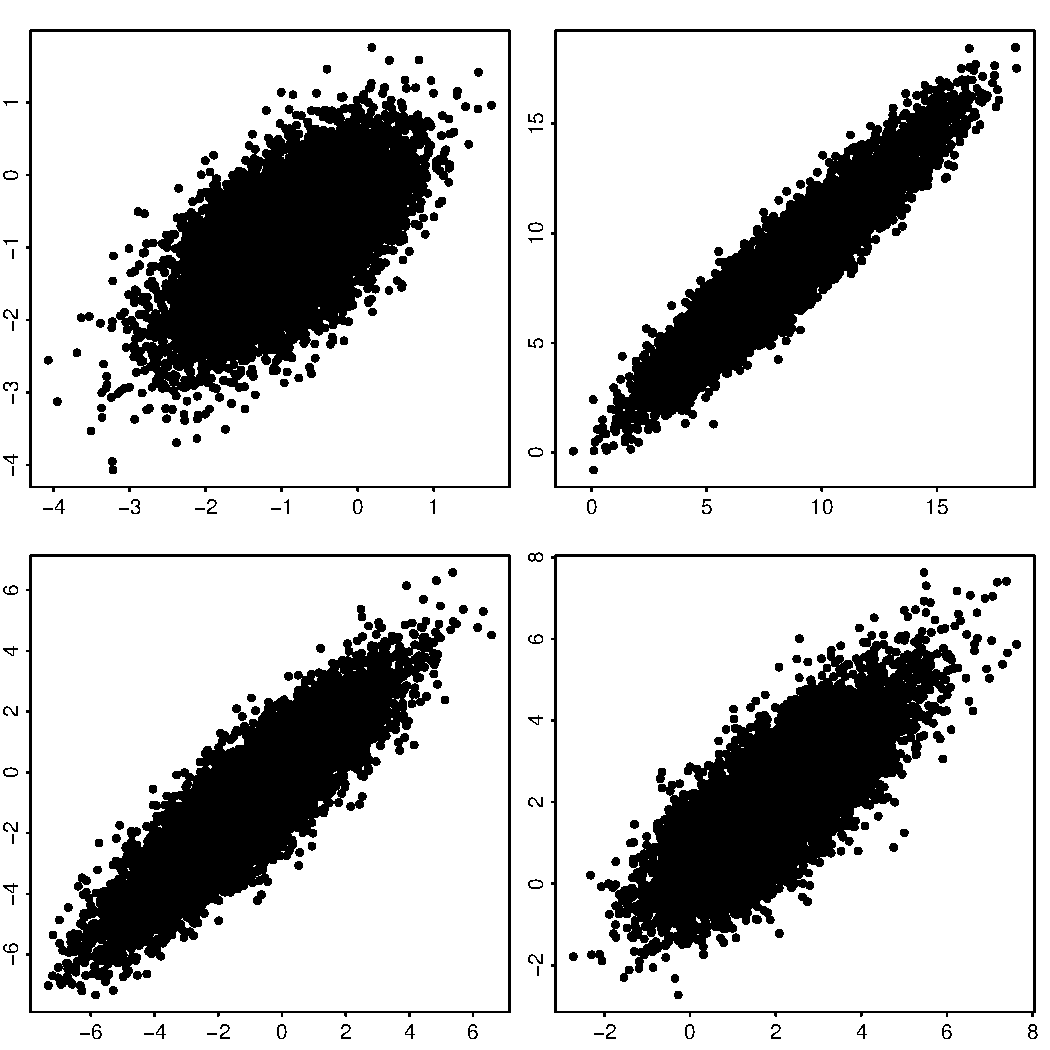
\includegraphics[width=.5\textwidth]{../figs/MH-autocorrelation-10shift1}
	 %=================
	  \onslide<6>
	  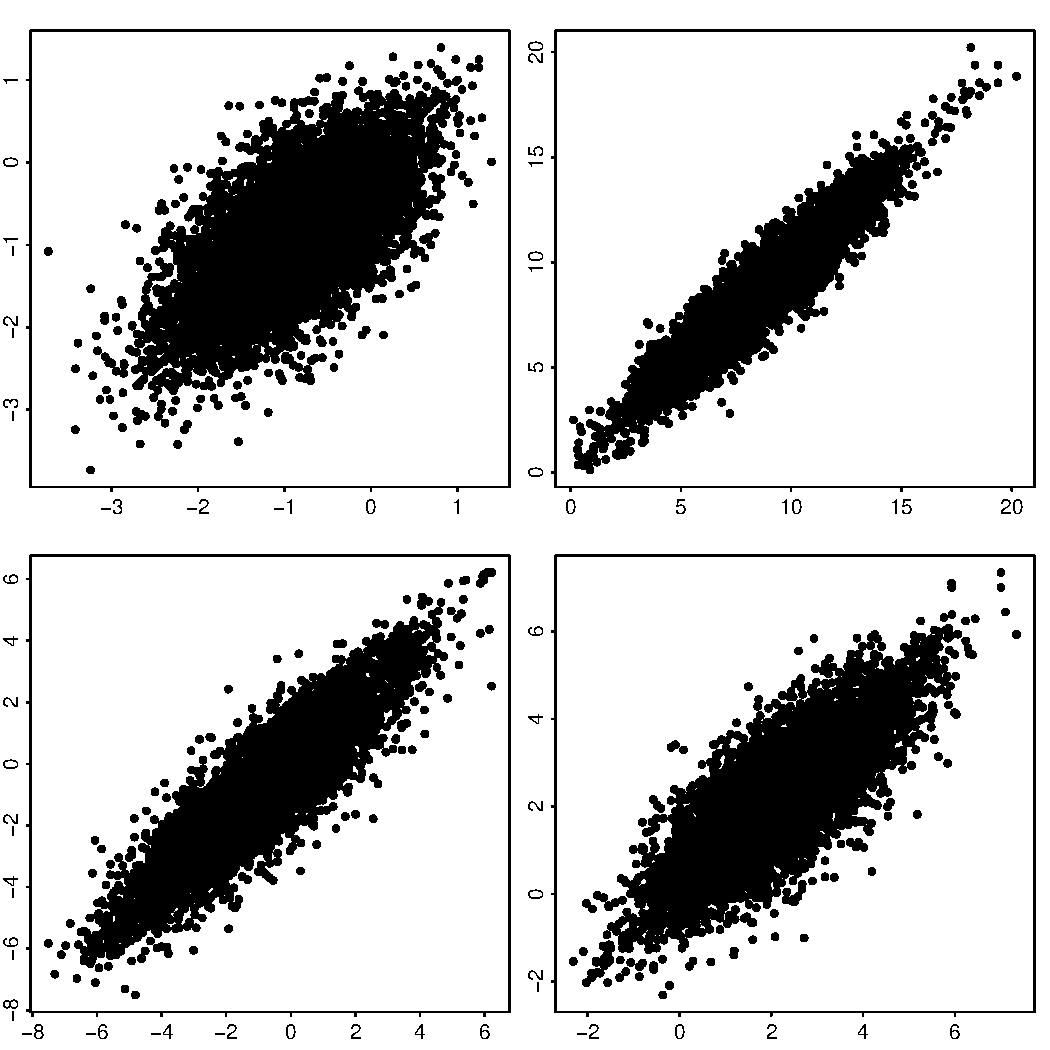
\includegraphics[width=.5\textwidth]{../figs/MH-autocorrelation-10shift5}
	 %=================
	  \onslide<7->
	  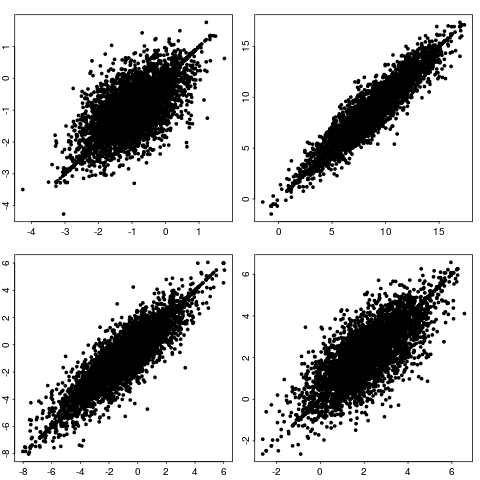
\includegraphics[width=.5\textwidth]{../figs/MH-autocorrelation-10shift10}
	 \end{overprint}
    \end{tabular}
  \end{tabular}
}

%====================================================================
\frame{ \frametitle{Gibbs sampler}

  \paragraph{Framework.} We do not know how to sample the whole vector $\thetabf$:
  $$
  p(\thetabf \gv \Ybf)
  $$
  but we may know how to sample each coordinate (conditional on the others):
  $$
  p(\theta_j \gv \Ybf, \thetabf_{-j})
  $$
  $\thetabf_{-j} = (\theta_1, \dots, \theta_{j-1}, \theta_{j+1}, \dots \theta_p)$.
  
  \pause \bigskip \bigskip
  \paragraph{Sampling a genotype.}
  \begin{itemize}
   \item Hard to sample a whole genotype (accounting for linkage disequilibrium)
   \item Easy to sample the genotype at one locus, conditional on the rest of the genotype
  \end{itemize}
}

%====================================================================
\frame{ \frametitle{Gibbs sampling for Bayesian inference}

  \paragraph{Algorithm.} Sample $\{\thetabf^b\}_{b=0 ,\dots B}$ as follows.
  \begin{itemize}
   \item \pause Start with $\thetabf^0$
   \item \pause At step $b$, for $j = 1, \dots p$, sample $\theta_j^b$:
   $$
   \theta_j^b \gv \Ybf, \theta_1^b, \dots, \theta_{j-1}^b, \theta_{j+1}^{b-1}, \dots, \theta_p^{b-1}
   $$
  \end{itemize}

  \pause \bigskip  \bigskip
  \paragraph{Property.}
  \begin{itemize}
   \item Obviously, $p(\thetabf \gv \Ybf)$ is a stationary distribution.
   \item Does not suffices to prove ergodicity.
  \end{itemize}
  }

% %====================================================================
% \frame{ \frametitle{Example: sampling allelic frequencies}
% 
%   \paragraph{Model.} 2 alleles / marker.
%   % Useless: conjugate prior!!!
%   \begin{itemize} 
%    \item $p$ loci, $n$ individuals, 
%    \item $Y_{ij} =$ genotype of individual $i$ at locus $j$ $\in \{0, 1\}$
%    \item $\thetabf = (\theta_y)_{y \in \{0, 1\}^p}$
%    \item Prior: $\thetabf \sim \Dcal(\dbf)$, $\dbf = (d_y)$
%   \end{itemize}
%   
%   }
